% ============================================================
% UGA-Themed Beamer Template (Clean MWE)
% ============================================================

\documentclass[aspectratio=169,professionalfonts]{beamer}

% ---------- COLORS (swap with official UGA hex if you like) ----------
\usepackage{xcolor}
\definecolor{UGARed}{HTML}{BA0C2F}   % Verify with brand guide
\definecolor{UGABlack}{HTML}{000000}
\definecolor{UGAGray}{HTML}{8A8D8F}

% ---------- THEME & PROGRESS DOTS ----------
\usetheme{default}
\useinnertheme{circles}
\useoutertheme[subsection=false]{miniframes}
\usefonttheme{professionalfonts}
\setbeamertemplate{navigation symbols}{}
% Head/foot colors
\setbeamercolor{subsection in head/foot}{fg=white,bg=UGARed}
\setbeamercolor{headline}{fg=white, bg=UGARed}

\setbeamercolor{section in head/foot}{fg=white,bg=UGARed}
\setbeamercolor{section in head/foot shaded}{fg=white,bg=UGARed}
\setbeamercolor{footline}{bg=UGABlack,fg=white}
\setbeamercolor{frametitle}{fg=UGABlack}
\setbeamercolor{title}{fg=UGABlack}
\setbeamercolor{normal text}{fg=UGABlack}
\setbeamercolor{structure}{fg=UGARed}

% --- HEADLINE: slide dots grouped by section ---
\setbeamersize{mini frame size=0.16cm,mini frame offset=0pt}
% Show section labels above the clickable slide dots.
\setbeamertemplate{section in head/foot}[default]
\setbeamertemplate{section in head/foot shaded}[default][75]
\setbeamertemplate{mini frame}{%
  \tikz[baseline=-0.5ex] \filldraw[draw=white,fill=white,line width=0.6pt] (0,0) circle (2pt);%
}
\setbeamertemplate{mini frame in current subsection}{%
  \tikz[baseline=-0.5ex] \filldraw[draw=white,fill=UGARed,line width=0.6pt] (0,0) circle (2pt);%
}
\setbeamertemplate{mini frame in other subsection}{%
  \usebeamertemplate{mini frame in current subsection}%
}
\setbeamertemplate{mini frame in other section}{%
  \usebeamertemplate{mini frame in current subsection}%
}
\setbeamertemplate{headline}{%
  \begin{beamercolorbox}[wd=\paperwidth]{headline}
    \vskip1ex
    \insertnavigation{\paperwidth}
    \vskip3ex
  \end{beamercolorbox}
}

% Simple footline with slide numbers
\setbeamertemplate{footline}{
  \leavevmode%
  \hbox{%
    \begin{beamercolorbox}[wd=\paperwidth,ht=2.5ex,dp=1ex,leftskip=1em,rightskip=1em]{footline}%
      \insertshortauthor{} \hfill \insertframenumber/\inserttotalframenumber
    \end{beamercolorbox}}%
}

% ---------- PACKAGES ----------
\usepackage{amsmath,amssymb,mathtools}
\usepackage{graphicx}
\usepackage{booktabs}
\usepackage{bbm}
\usepackage{array}
\usepackage{adjustbox}
\usepackage{hyperref}
\usepackage{tikz}
\usetikzlibrary{arrows.meta, positioning}
\usepackage{tcolorbox}
\usepackage{eurosym}
\usepackage{threeparttable}
% ---------- METADATA (fill these later) ----------
\title{Optimal Dynamic Pricing With Preferences for Novelty}
\subtitle{}
\author{Tate Mason}
\institute{The University of Georgia}
\date{\today}

% ---------- MACROS ----------
% Numbered equation with label
\newcommand{\beq}[1]{\begin{equation}\label{#1}}
\newcommand{\eeq}{\end{equation}}
% Accent color highlight
\newcommand{\hl}[1]{\textbf{\textcolor{UGARed}{#1}}}
% Simple figure placeholder macro
\newcommand{\figph}[2][0.9\linewidth]{%
  \begin{figure}
    \centering
    \fbox{\rule{0pt}{0.55#1}\rule{#1}{0pt}}%
    \caption{#2}
  \end{figure}
}

% ============================================================

% Keep navigation links in the theme's white foreground on the red header.
\hypersetup{colorlinks=true, linkcolor=., urlcolor=UGARed}


% Short-version navigation only. Original frame content is preserved verbatim.
\newcommand{\shortbuttons}{}
\newcommand{\shortmaincount}{37}
\newif\ifshortappendix
\shortappendixfalse
\setbeamertemplate{footline}{%
  \leavevmode\vbox{\hbox{%
  \begin{beamercolorbox}[wd=\paperwidth,ht=3.8ex,dp=.6ex,rightskip=1em]{normal text}%
    \hfill{\scriptsize\shortbuttons}
  \end{beamercolorbox}}%
  \hbox{\begin{beamercolorbox}[wd=\paperwidth,ht=2.5ex,dp=1ex,leftskip=1em,rightskip=1em]{footline}%
    \insertshortauthor{}\hfill
    \ifshortappendix Appendix\else\insertframenumber/\shortmaincount\fi
  \end{beamercolorbox}}}%
}


\begin{document}

% Original numbered slide 0
\gdef\shortbuttons{}
\begin{frame}[plain,noframenumbering,label=short-0]
  \titlepage
\end{frame}


\section{Introduction}

% Original numbered slide 1
\gdef\shortbuttons{}
\begin{frame}[label=short-1]{Motivation}
  \begin{itemize}
    \item Firms have more access than ever to consumer information
    \item Allows for targeted discounting based on preferences derived from repeat interactions
    \item Targeted discounts allow firms to steer consumers toward particular products.
  \end{itemize}
  \begin{tcolorbox}
    How do firms price based on repeated interactions with consumers and how are profits affected?
  \end{tcolorbox}
\end{frame}


% Original numbered slide 2
\gdef\shortbuttons{}
\begin{frame}[label=short-2]{Research Question}
  \begin{tcolorbox}
    How can firms price discriminate via consumer preferences for novelty and habit and how much is information about these preferences worth?
  \end{tcolorbox}
  How do I answer?
  \begin{itemize}
    \item Solve a theoretical model to understand firm's behavior
    \item Estimate consumer's preferences with Nielsen data, recovering the distribution of novelty/habit preferences
    \item Use the estimated distribution in the pricing model to understand how firm's revenues are impacted by this sort of targeting
  \end{itemize}
\end{frame}


% Original numbered slide 3
\gdef\shortbuttons{}
\begin{frame}[label=short-3]{Literature}
  \begin{columns}[T]
    \begin{column}{0.48\textwidth}
      \textbf{Targeting:}
      \begin{itemize}
        \item Dub\'e (2008)
        \item Dub\'e et. al (2022) 
        \item Anand \& Shachar (2009)
        \item Karle \& Reisinger (2024)
        \item Durrmeyer, Fournel, Samano (2026)
      \end{itemize}
    \end{column}
    \begin{column}{0.48\textwidth}
      \textbf{Estimating preferences for novelty:}
      \begin{itemize}
        \item Dub\'e (2004)
        \item Dub\'e et. al (2021)
        \item Chintagunta (1999)
        \item Lattin (1987)
        \item McAllister (1982)
        \item Ackerberg (2003)
      \end{itemize}
    \end{column}
  \end{columns}
\end{frame}


\section{Motivation from Data}

% Original numbered slide 4
\gdef\shortbuttons{\hyperlink{short-5}{\beamergotobutton{Flavor Popularity}}}
\begin{frame}[label=short-4]{HHI}
  \centering
    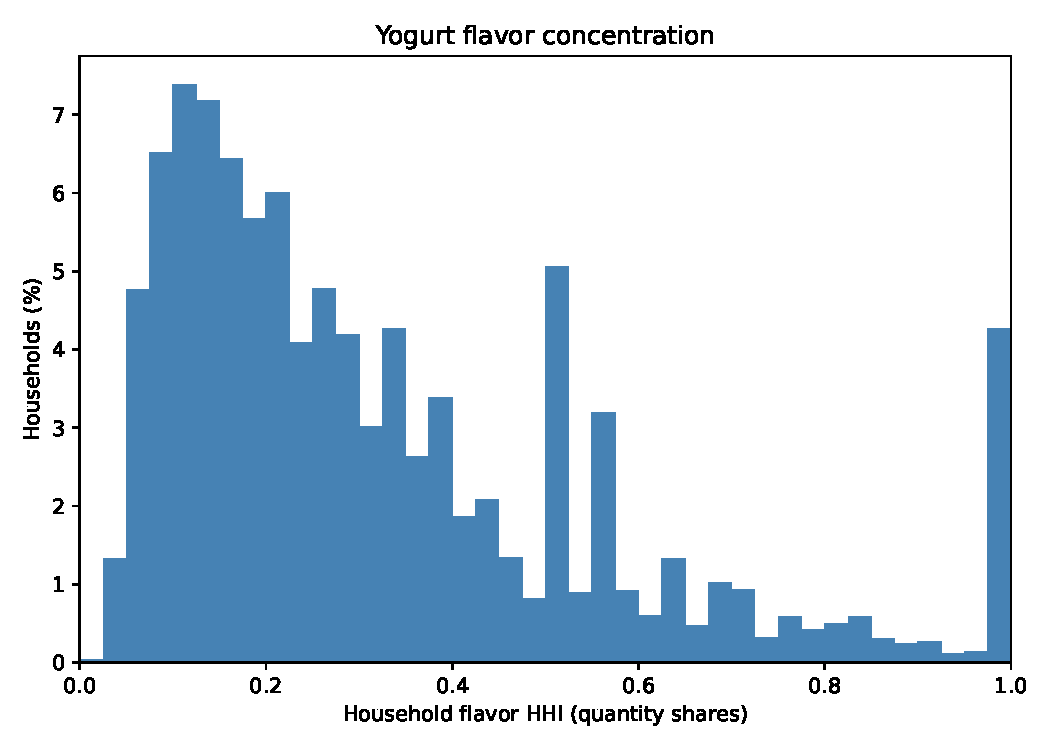
\includegraphics[width=.95\textwidth,height=.74\textheight,keepaspectratio]{../writeup/1108_writeup/assets/results/summary_statistics/flavor_hhi_histogram.pdf}
\end{frame}


\section{Supply Theory}

% Original numbered slide 6
\gdef\shortbuttons{}
\begin{frame}[label=short-6]{Supply Setting}
  \begin{itemize}
    \item Monopolistic firm producing a single product $j$
    \item Firm is profit maximizing, setting prices according to that objective
    \item A consumer is born into the world with a type $r\in\{H,L\}$, determining how much utility they derive from switching and an initial state $h_0\in\{0,j\}$
    \item Consumers live for two periods, purchasing the inside good or opting for the outside good in each period
    \item The firm knows initial states and types, setting prices to individual consumers by type and history
  \end{itemize}
\end{frame}


% Original numbered slide 7
\gdef\shortbuttons{}
\begin{frame}[label=short-7]{Consumer's Problem}
  \begin{tcolorbox}[
    boxsep=0pt,
    left=2pt, right=2pt,
    top=1pt, bottom=1pt,
    before skip=2pt, after skip=2pt
    ]
    \setlength{\abovedisplayskip}{2pt}
    \setlength{\belowdisplayskip}{2pt}
    \begin{gather*}
      V^{inside}_{jt} = \underbrace{\beta}_{\text{Constant}} + \overbrace{\gamma_r\mathbbm{1}\{h=0\}}^{\text{Utilty from Switching}} - \underbrace{\alpha p_t(h)}_{\text{Price Disutility}}, \ V^{Outside}_{0t} = \underbrace{\gamma_r\mathbbm{1}\{h=j\}}_{\text{Utility from Switching}} \\
      v_t(x) = V_{jt}^{inside} - V_{0t}^{outside} = \beta + \underbrace{\gamma[\mathbbm{1}\{h=0\} - \mathbbm{1}\{h=j\}]}_{q(h)} - \alpha p_t(h)
    \end{gather*}
  \end{tcolorbox}
  \begin{itemize}\setlength{\itemsep}{2pt}
    \item Prices, set by the firm, and switching utility depend on history $h=x_{t-1}$
    \item Utility for the outside good is normalized to zero
  \end{itemize}
\end{frame}


% Original numbered slide 8
\gdef\shortbuttons{}
\begin{frame}[label=short-8]{Firm's Problem}
  \begin{tcolorbox}
    [
    boxsep=0pt,
    left=2pt, right=2pt,
    top=1pt, bottom=1pt,
    before skip=2pt, after skip=2pt
    ]
    \setlength{\abovedisplayskip}{2pt}
    \setlength{\belowdisplayskip}{2pt}
    \begin{gather*}
      \pi_t(h) = \max_{p_t(h)} s_t(h)[p_t(h) - c] \\ 
      \Pi(h) = \underbrace{s_1(h)(p_1(h) - c)}_{\text{Margin in Period 1}} + \underbrace{\delta\{s_1(h)\pi_2(j) + (1-s_1(h))\pi_2(0)\}}_\text{{Continuation Value}} 
    \end{gather*}
  \end{tcolorbox}
  \begin{itemize}
    \item Firm profits are comprised of period one margins, given history of consumption, and the value of that consumer in the different states in period two
    \item The firm will set prices according to consumer type and history to maximize expected profit
  \end{itemize}
\end{frame}


% Original numbered slide 10
\gdef\shortbuttons{\hyperlink{short-9}{\beamergotobutton{Terminal FOC}}\hspace{.35em}\hyperlink{short-11}{\beamergotobutton{Comparative statics}}\hspace{.35em}\hyperlink{short-52}{\beamergotobutton{Elasticities}}}
\begin{frame}[label=short-10]{First Period Optimization}
  \begin{tcolorbox}
    [
    boxsep=0pt,
    left=2pt, right=2pt,
    top=1pt, bottom=1pt,
    before skip=2pt, after skip=2pt
    ]
    \setlength{\abovedisplayskip}{2pt}
    \setlength{\belowdisplayskip}{2pt}
    \begin{align*}
      \frac{d\Pi}{d p_1(h_0)} &= s_1 + \frac{\partial}{\partial p_1(h)}s_1(h_0)[p_1(h_0) - c + \delta(\pi_2(j) - \pi_2(0))] \\
      p_1^*(h_0) &= c + \frac{1}{\alpha(1-s_1^*(h_0))} - \delta(\pi_2(j) - \pi_2(0)) \\
      \Pi^*(h) &= \delta\pi_2(0) + \frac{s_1^*(h_0)}{\alpha(1-s_1^*(h_0))}
    \end{align*}
  \end{tcolorbox}
\end{frame}


% Original numbered slide 14
\gdef\shortbuttons{\hyperlink{short-12}{\beamergotobutton{Calibration}}\hspace{.35em}\hyperlink{short-13}{\beamergotobutton{Table}}\hspace{.35em}\hyperlink{short-15}{\beamergotobutton{Profit}}\hspace{.35em}\hyperlink{short-16}{\beamergotobutton{Price ratio}}\hspace{.35em}\hyperlink{short-17}{\beamergotobutton{Discussion}}}
\begin{frame}[label=short-14]{Optimal Prices}
  \centering
  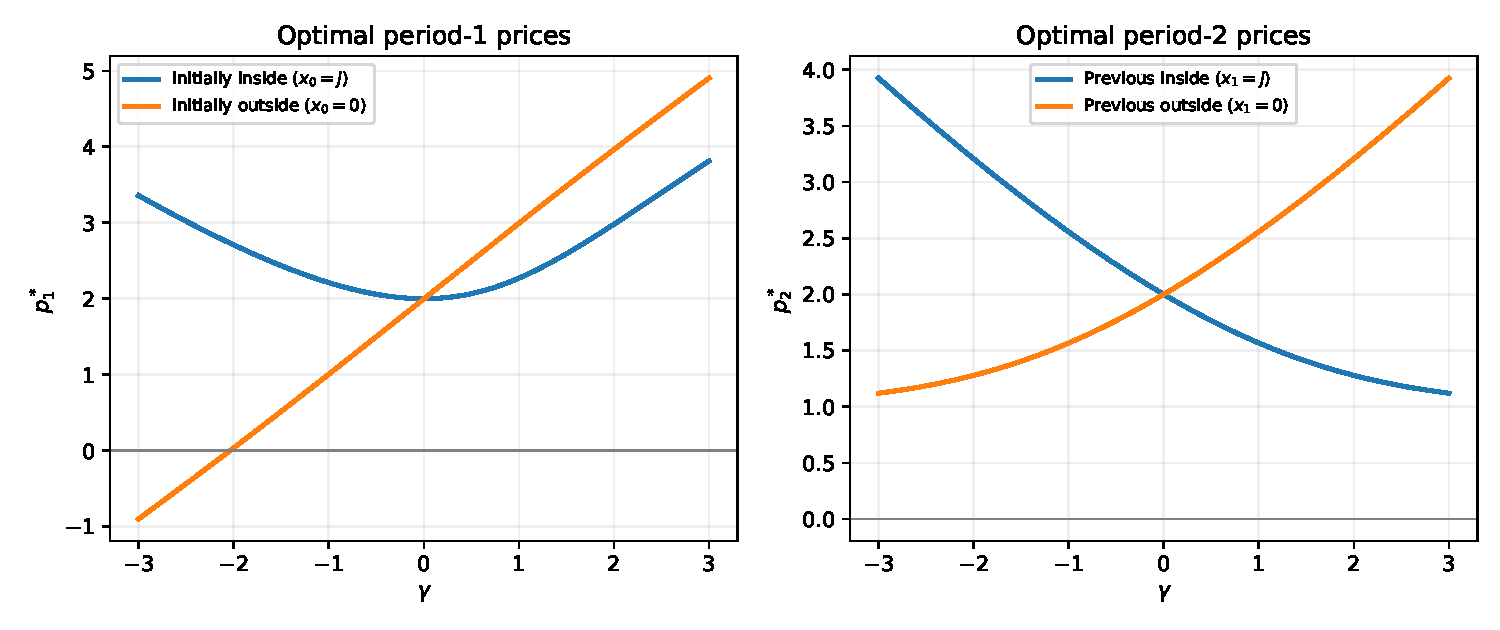
\includegraphics[width=0.85\textwidth]{assets/theory_delta1/optimal_prices_by_gamma.pdf}
\end{frame}


% Theory plots regenerated at delta=1.
\gdef\shortbuttons{\hyperlink{short-14}{\beamergotobutton{Optimal prices}}\hspace{.35em}\hyperlink{short-15}{\beamergotobutton{Profit detail}}\hspace{.35em}\hyperlink{short-16}{\beamergotobutton{Price-ratio detail}}}
\begin{frame}[label=short-prices-profit]{Optimal Price Ratios and Profit}
  \centering
  \begin{columns}[T,onlytextwidth]
    \begin{column}{.49\textwidth}
      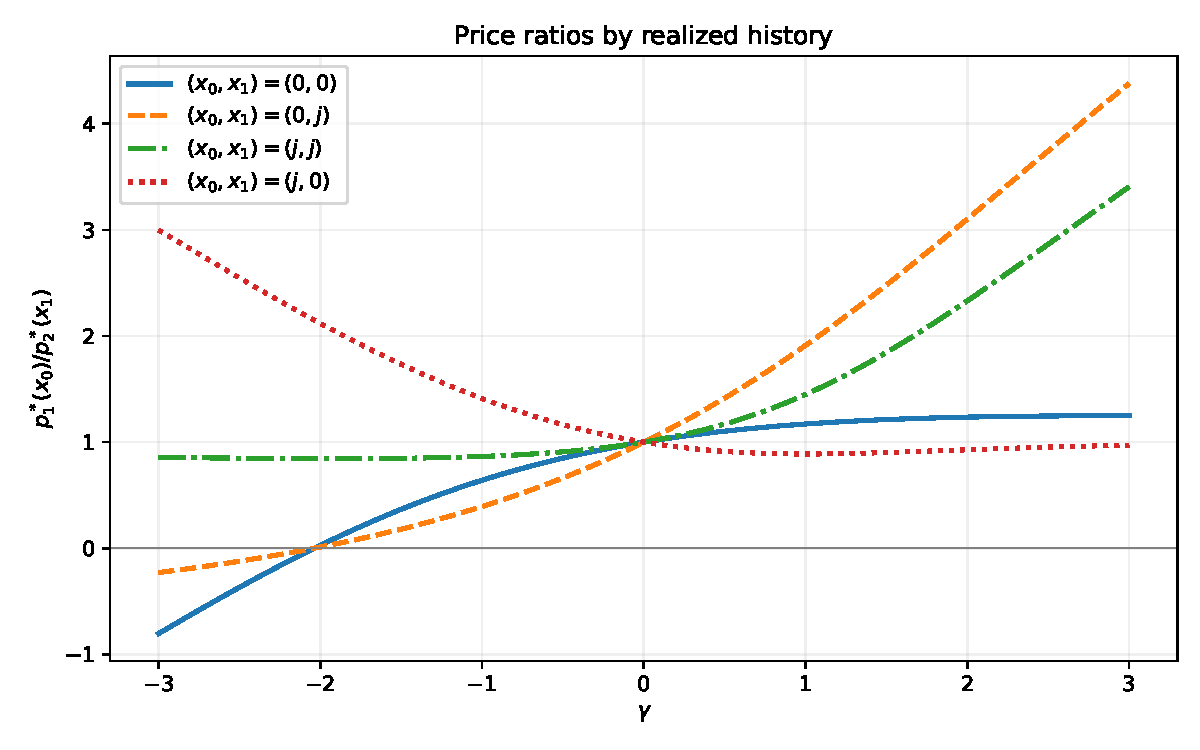
\includegraphics[width=\linewidth,height=.66\textheight,keepaspectratio]{assets/theory_delta1/all_state_price_ratios.pdf}
    \end{column}
    \begin{column}{.49\textwidth}
      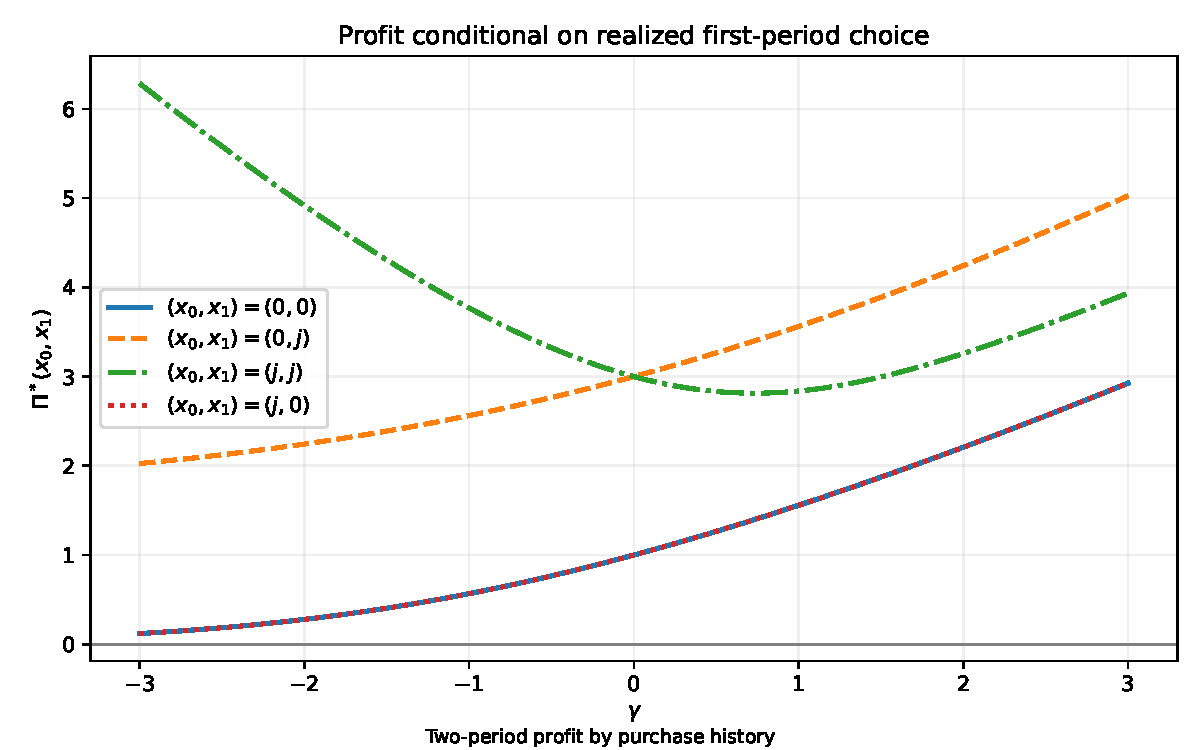
\includegraphics[width=\linewidth,height=.66\textheight,keepaspectratio]{assets/theory_delta1/all_state_realized_profit.pdf}
    \end{column}
  \end{columns}
  \vspace{.3em}
  {\footnotesize $\delta=1$: no discounting. Flavor is $j$; outside is everything except that flavor.}
\end{frame}


% Original numbered slide 18
\gdef\shortbuttons{}
\begin{frame}[label=short-18]{Information Friction: Fixed Beliefs about Switching Type}
 \begin{itemize}
 \item Initial purchase history is observed.
 \item $\gamma_L=-1.25$, $\gamma_0=0$, $\gamma_H=1.25$.
 \item $\Pr(\gamma=\gamma_r)=\mu_r$, $r\in\{H,0,L\}$. Equal case: $\mu_r=0.33$.
 \item Other cases: each permutation of $(0.50,0.25,0.25)$.
 \item Type probabilities stay fixed in both periods, after either purchase outcome.
 \item Offers depend on observed history; there is no learning about type.
 \end{itemize}
 \begin{align*}
 s_t(h)&=\sum_r\mu_r\,s_t(h\mid\gamma_r),\\
 \pi_2(h)&=\max_{p_2(h)}s_2(h)\,[p_2(h)-c].
 \end{align*}
\end{frame}


% Original numbered slide 20
\gdef\shortbuttons{\hyperlink{short-19}{\beamergotobutton{Profit levels}}\hspace{.35em}\hyperlink{short-53}{\beamergotobutton{Price paths}}\hspace{.35em}\hyperlink{short-54}{\beamergotobutton{Price paths}}}
\begin{frame}[label=short-20]{Personalized vs Common Pricing}
\centering
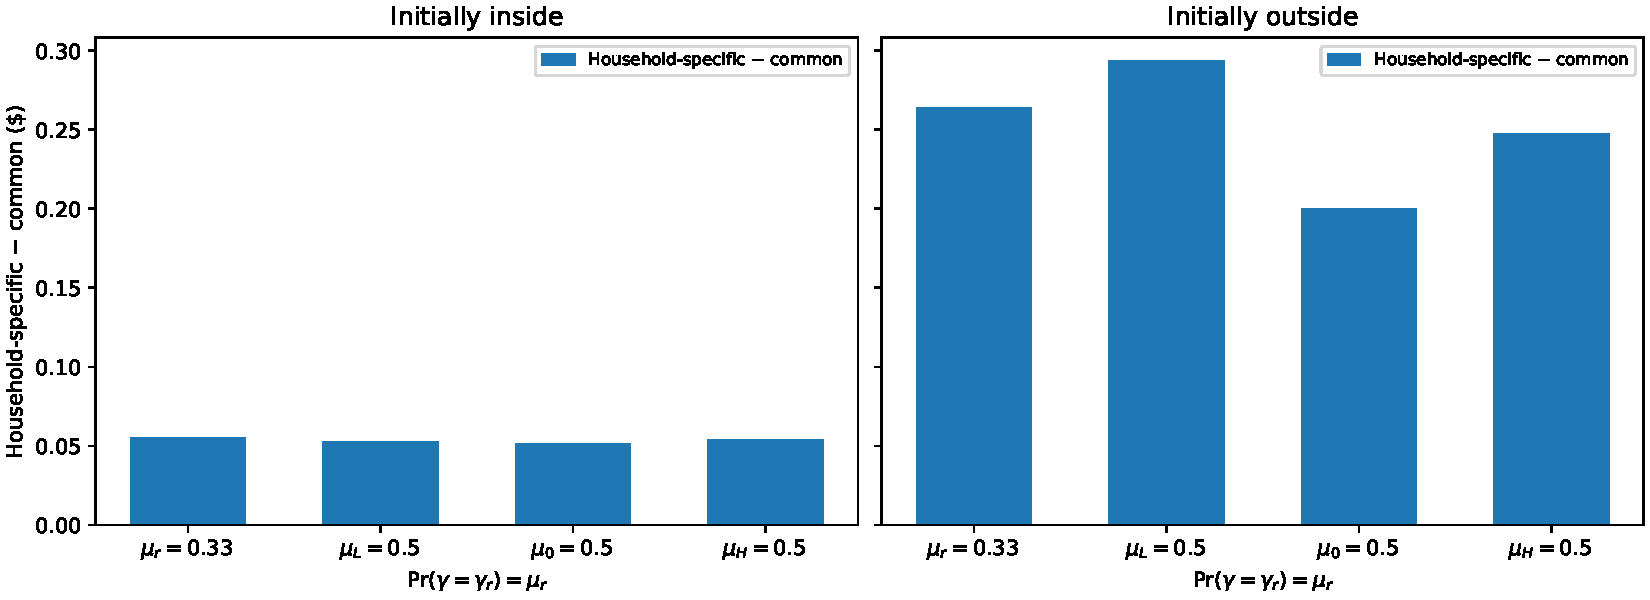
\includegraphics[width=.98\textwidth,height=.78\textheight,keepaspectratio]{assets/theory_delta1/gamma_uncertainty/information_value.pdf}
\end{frame}


\section{Data}

% Original numbered slide 21
\gdef\shortbuttons{\hyperlink{short-22}{\beamergotobutton{Activity}}}
\begin{frame}[label=short-21]{Data Sources}
  \textbf{Nielsen HomeScan}
  \begin{itemize}
    \item Provides household level purchase data
    \item Covers years 2006-2015
    \item Products chosen, quantity chosen, timing of trips
  \end{itemize}
  \textbf{Nielsen RetailScan}
  \begin{itemize}
    \item Provides store level product data
    \item For specified product category: prices, markets, product attributes
  \end{itemize}
  \textbf{Sample Description}
  \begin{itemize}
    \item Must be single-person household 
    \item Must be seen at least 2 times
    \item Purchases must be made at Nielsen store (prices available)
    \item Flavor attribute must be present
  \end{itemize}
\end{frame}


% Original numbered slide 23
\gdef\shortbuttons{}
\begin{frame}[label=short-23]{Sample Statistics: Demographics}
  \centering
  \begin{adjustbox}{max totalsize={\textwidth}{.83\textheight},center}
    \begin{minipage}{\textwidth}
      % Aggregate sources: full_panel_overview.tex, matched_yogurt_overview.tex,
% full_panel_household_size.tex, and matched_yogurt_household_size.tex.
% Requires \usepackage{booktabs}.
\begin{table}[htbp]\centering\small
\centering
\caption{Summary statistics: full sample and yogurt sample}
\label{tab:full-panel-vs-yogurt}
\begin{adjustbox}{max width=\linewidth}
\begin{tabular}{lrr}
\toprule
 & Full sample & Yogurt sample \\
\midrule
\multicolumn{3}{l}{\textit{Sample and purchase activity}} \\
Households & 37,827 & 15,106 \\
Mean observed panel years & 3.96 & 3.16 \\
Mean trips per household & 493.13 & 20.26 \\
Mean trips per approximate observed week & 2.27 & 0.11 \\
Mean distinct UPCs per household & 1,178.31 & 13.89 \\
Mean purchase lines per household & 3,397.64 & 45.15 \\
Mean packages per household & 4,669.07 & 93.77 \\
Mean head age (category code) & 6.96 & 7.01 \\
Mean household income (category code) & 16.18 & 17.06 \\
Race: White (\%) & 80.33 & 81.58 \\
Race: Black (\%) & 12.81 & 12.15 \\
Race: Asian (\%) & 1.57 & 1.57 \\
Race: Other (\%) & 2.19 & 2.11 \\
Hispanic (\%) & 3.10 & 2.59 \\
\bottomrule
\end{tabular}
\end{adjustbox}
\end{table}

    \end{minipage}
  \end{adjustbox}
\end{frame}

% Original numbered slide 24
\gdef\shortbuttons{}
\begin{frame}[label=short-24]{Switching Stats}
    \centering
    \resizebox{\textwidth}{!}{%
    \begin{minipage}{\textwidth}
      \begin{table}
\caption{Matched yogurt sample: purchase dynamics}
\begin{tabular}{lr}
\toprule
metric & value \\
\midrule
Matched households & 15106.00 \\
Observed yogurt purchase weeks & 282648.00 \\
Mean flavors bought per household & 1.93 \\
Mean household flavor HHI (0 to 1) & 0.78 \\
Mixed-flavor weeks (\%) & 17.45 \\
Weeks above seven packages (\%) & 21.72 \\
Eligible adjacent single-flavor week pairs & 48166.00 \\
Switch rate in eligible pairs (\%) & 12.85 \\
Mean single-flavor spell length (consecutive calendar weeks) & 1.22 \\
Median gap between purchase weeks & 3.00 \\
\bottomrule
\end{tabular}
\end{table}

    \end{minipage}%
    }
\end{frame}


% Original numbered slide 25
\gdef\shortbuttons{}
\begin{frame}[label=short-25]{Persistence Across Aggregated Flavor Groups}
  \centering
  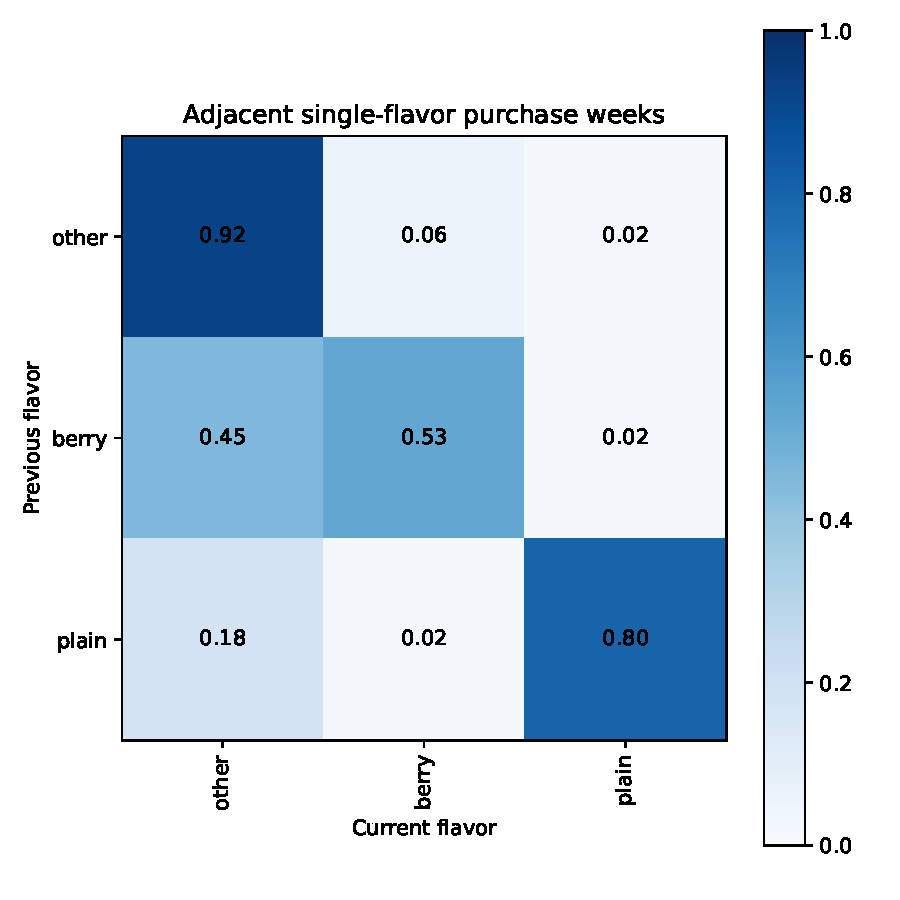
\includegraphics[height=0.69\textheight]{../writeup/1108_writeup/assets/results/summary_statistics/aggregated_flavors/flavor_transitions.pdf}
  \par\small Plain repeats in approximately 80\% of eligible transitions, versus 53\% for berry.
\end{frame}


\section{Demand Estimation}

% Original numbered slide 26
\gdef\shortbuttons{}
\begin{frame}[label=short-26]{Demand Setting and Objective}
  \begin{itemize}
    \item Consumers can either purchase the inside good, a flavor of yogurt, or the outside good, not yogurt 
    \item Following Nevo (2001), a week contains seven choice opportunities with observed flavor purchases treated as fulfilling an opportunity 
    \item Define outside good as $\max(0, 7-\sum_j x_{jt})$, or the difference in purchases and a full week
    \item Consumers differ in preferences for novelty and price sensitivity, but derive the same base utility from the three flavor categories
    \item Goal: \textcolor{red}{Recover distribution of novelty preferences}
  \end{itemize}
\end{frame}


% Original numbered slide 27
\gdef\shortbuttons{}
\begin{frame}[label=short-27]{Demand Model}
\begin{tcolorbox}[boxsep=0pt,left=2pt,right=2pt,top=2pt,bottom=2pt]
    \setlength{\abovedisplayskip}{3pt}
    \setlength{\belowdisplayskip}{3pt}
    \[
    U_{ijt}=\overbrace{\beta_0}^{\text{Constant}}
      +\underbrace{\beta_jX_{jt}}_{\text{Flavor specific constant}}
      +\overbrace{\gamma_iN_{ijt}+\phi_iH_{ijt}}^{\text{Preferences for novelty/habit}}
      +\underbrace{\alpha_ip_{jt}}_{\text{Price disutility}}
      +\overbrace{\varepsilon_{ijt}}^{\text{T1EV}}
    \]
  \end{tcolorbox}
  \medskip
  Normalize outside option to zero s.t. $U_{i0t}=\varepsilon_{i0t}$
\end{frame}

\gdef\shortbuttons{}
\begin{frame}[label=short-history]{Novelty and Habit}
  \setlength{\abovedisplayskip}{4pt}
  \setlength{\belowdisplayskip}{4pt}
  \[
  w_{ijt}=y_{ijt}/\!\sum_k y_{ikt}
  \]
  \textbf{Novelty}
  \[
  N_{ijt}=\begin{cases}
    1-w_{ij,t-1},&\text{prior calendar week observed},\\
    0,&\text{otherwise}.
  \end{cases}
  \]
  $N_{ijt}$ is the prior week's purchase share in flavors other than $j$

  \medskip
  \textbf{Habit}
  \[
  H_{ijt}=\sum_{s<t}w_{ijs}
  \]
  $H_{ijt}$ accumulates prior weekly own-flavor purchase shares
\end{frame}


% Original numbered slide 29
\gdef\shortbuttons{\hyperlink{short-28}{\beamergotobutton{Probabilities}}\hspace{.35em}\hyperlink{short-55}{\beamergotobutton{Price controls}}\hspace{.35em}\hyperlink{short-56}{\beamergotobutton{Controlled estimates}}\hspace{.35em}\hyperlink{short-61}{\beamergotobutton{First stages}}}
\begin{frame}[label=short-29]{Estimation}
  \begin{tcolorbox}
    [
    boxsep=0pt,
    left=2pt, right=2pt,
    top=1pt, bottom=1pt,
    before skip=2pt, after skip=2pt
    ]
    \setlength{\abovedisplayskip}{2pt}
    \setlength{\belowdisplayskip}{2pt}
    \begin{align*}
      P_i(\theta) &= \int P(y_i\mid\nu,\theta)\ \phi(\nu)\,d\nu \\
      \widehat P_i(\theta) &= \frac{1}{128}\sum_{r=1}^{128}\prod_{t=1}^{T_i}P_(y_i\mid\nu_{ir}, \theta)\qquad\nu_{ir}\sim\mathcal N(0, I) \\
      Q_{128}(\theta) &= -\sum_{i=1}^N\log\widehat P_i(\theta)
    \end{align*}
  \end{tcolorbox}
  \begin{itemize}
    \item $\nu_i$ captures unobserved heterogreneity, $y_{it}$ represents observed choice, $\theta = \{\beta, \gamma, \phi, \alpha\}$ is the vector of heterogeneous demand parameters
    \item 128 draws per household from a normal distribution
    \item 3 starts at different starting values, keep lowest objective 
    \item Minimize negative log-likelihood
  \end{itemize}
\end{frame}


% Original numbered slide 32
\gdef\shortbuttons{\hyperlink{short-30}{\beamergotobutton{Estimates}}\hspace{.35em}\hyperlink{short-33}{\beamergotobutton{Discussion}}}
\begin{frame}[label=short-32]{Distributions}
  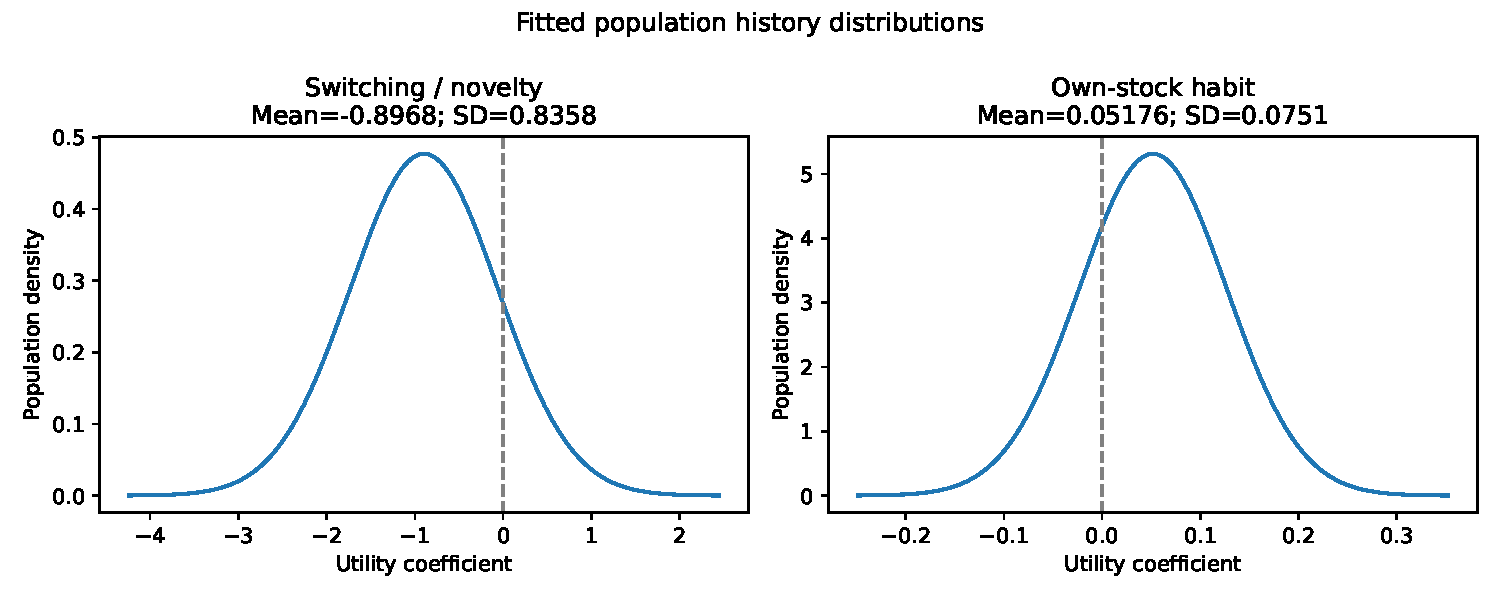
\includegraphics[width=0.99\textwidth]{../writeup/1108_writeup/assets/results/demand/history_distributions.pdf}
\end{frame}


% Original numbered slide 31
\gdef\shortbuttons{\hyperlink{short-62}{\beamergotobutton{Controlled WTP}}}
\begin{frame}[label=short-31]{Implied Willingness to Pay}
  \centering
  \begin{table}[htbp]\centering\small
\caption{Implied willingness to pay without price controls}
\label{tab:wtp-demand}
\begin{adjustbox}{max width=\linewidth}
\begin{tabular}{lrr}\toprule
Utility term & Mean WTP & Population SD\\\midrule
Inside constant $\beta_0$ & 2.7474 & 2.7716 \\
Berry vs. other & -1.4085 & 1.4210 \\
Plain vs. other & -0.6137 & 0.6192 \\
novelty & -1.7451 & 3.1116 \\
own stock & 0.0833 & 0.2647 \\
\bottomrule\end{tabular}
\end{adjustbox}
\end{table}

  \begin{itemize}
    \item Would need to be subsidized to switch, though lots of variation
    \item Willing to pay to continue consuming their same product
  \end{itemize}
\end{frame}


\section{Pricing Exercise}

% Original numbered slide 34
\gdef\shortbuttons{}
\begin{frame}[label=short-34]{Connecting Supply and Demand}
  \begin{columns}[T]
    \begin{column}{0.48\textwidth}
      \textbf{Supply Theory}
      \begin{itemize}
        \item Today's pricing offer changes tomorrow's demand
        \item Single product firm pricing to attract customers against outside option
        \item Maintain two-period timing with initial state
      \end{itemize}
    \end{column}
    \begin{column}{0.48\textwidth}
      \textbf{Empirical Demand}
      \begin{itemize}
        \item Employ estimated preference for novelty
        \item Access observed purchase histories
        \item Novelty and habit both enter demand
      \end{itemize}
    \end{column}
  \end{columns}
  \begin{tcolorbox}
    How well does the theory map to what is observed in the data?
  \end{tcolorbox}
\end{frame}


% Original numbered slide 35
\gdef\shortbuttons{}
\begin{frame}[label=short-35]{Procedure}
  \begin{itemize}
    \item Recover household type from observed purchase history and treat estimated type as known to firm
    \item Use initial purchase $y_{i1}$ to determine "initial state", $h_0$
    \item Separate high and low types as the 75th and 25th percentiles, respectively
    \item Compare common pricing and personalized pricing over two periods
    \item Focus on berry and plain to maintain parity with the theoretical model and avoid aggregate weighting
    \item Use the estimated demand model to choose the initial offer $p_1$ and then the terminal offer $p_2$ after observing the first-period choice
  \end{itemize}
\end{frame}


% Original numbered slide 40
\IfFileExists{assets/pricing/plain/pricing_policy_benchmarks.pdf}{
\gdef\shortbuttons{}
\begin{frame}[label=short-40]{Pricing Comparison: Plain}
  \centering
  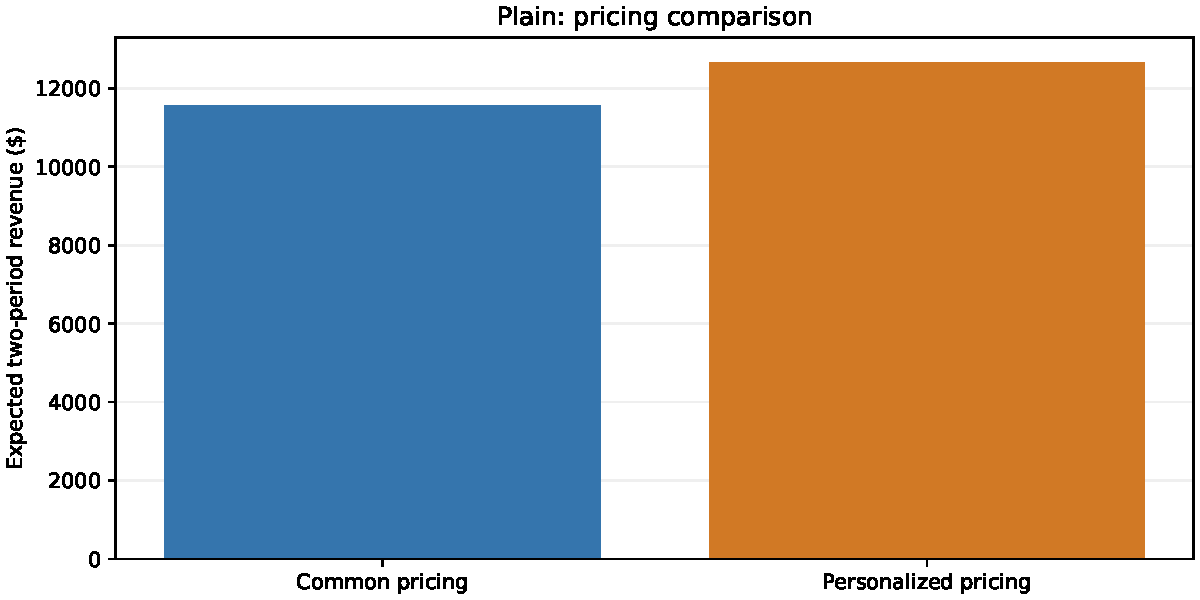
\includegraphics[width=0.85\textwidth]{assets/pricing/plain/pricing_policy_benchmarks.pdf}
\end{frame}
}{}


% Original numbered slide 41
\IfFileExists{assets/pricing/berry/pricing_policy_benchmarks.pdf}{
\gdef\shortbuttons{}
\begin{frame}[label=short-41]{Pricing Comparison: Berry}
  \centering
  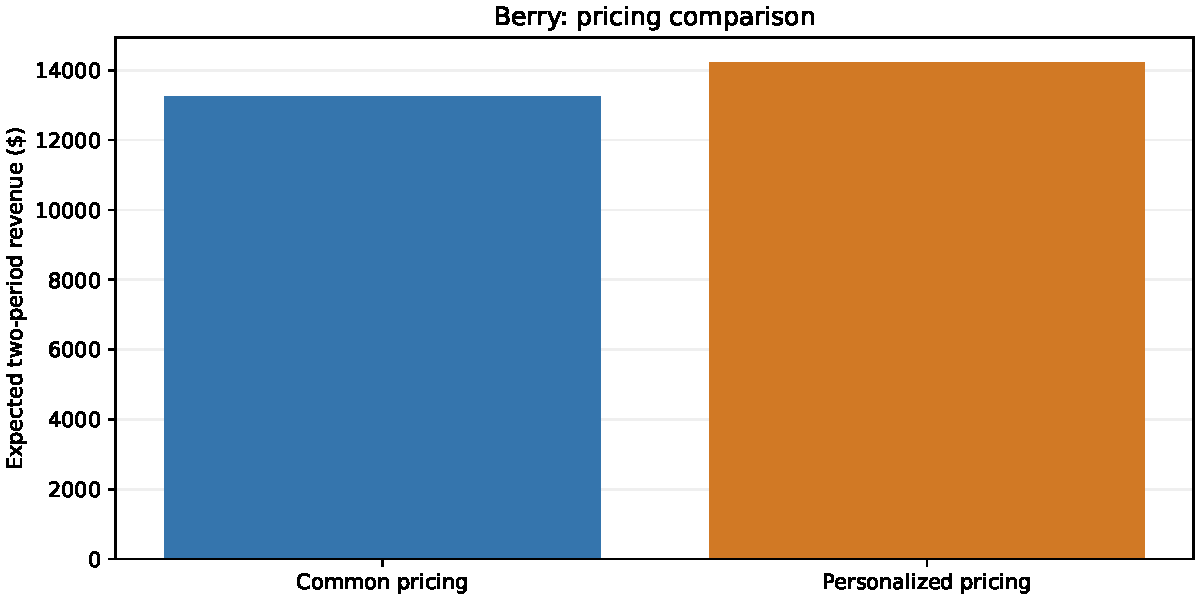
\includegraphics[width=0.85\textwidth]{assets/pricing/berry/pricing_policy_benchmarks.pdf}
\end{frame}
}{}


% Original numbered slide 42
\gdef\shortbuttons{\hyperlink{short-38}{\beamergotobutton{Berry offers}}\hspace{.35em}\hyperlink{short-39}{\beamergotobutton{Plain offers}}}
\begin{frame}[label=short-42]{Plain: Price Paths}
  \centering
  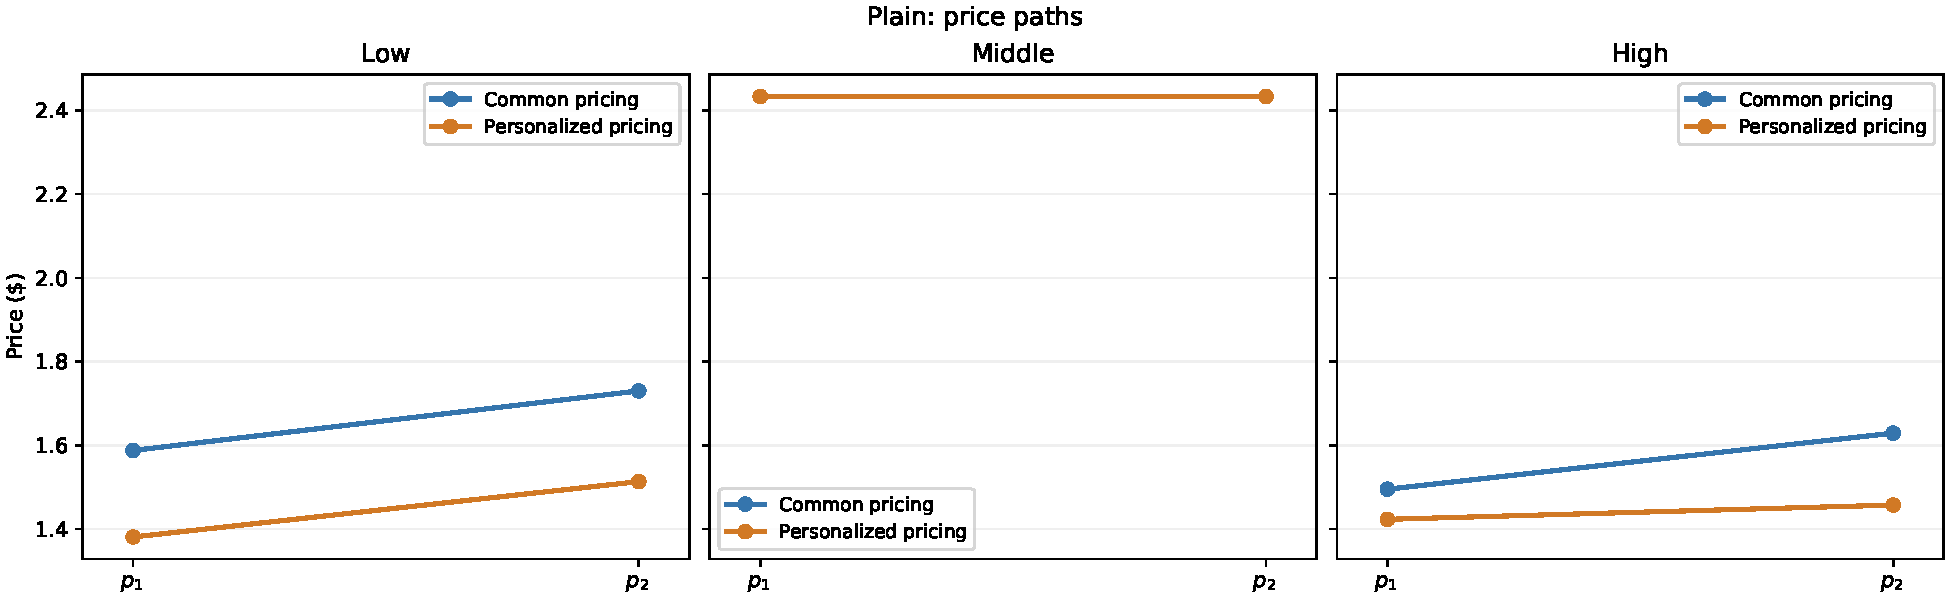
\includegraphics[width=0.95\textwidth]{assets/pricing/plain/pricing_mechanism.pdf}
\end{frame}




% Original numbered slide 44
\gdef\shortbuttons{\hyperlink{short-36}{\beamergotobutton{Berry types}}\hspace{.35em}\hyperlink{short-37}{\beamergotobutton{Plain types}}}
\begin{frame}[label=short-44]{Comparison}
  \centering
  \begin{tabular}{llrr}\toprule
Flavor & Policy & Revenue & Gain (\%)\\\midrule
Plain & Common pricing & 11,559.5 & 0.00\\
Plain & Personalized pricing & 12,655.8 & 9.48\\
Berry & Common pricing & 13,257.2 & 0.00\\
Berry & Personalized pricing & 14,219.7 & 7.26\\
\bottomrule\end{tabular}

\end{frame}


% Original numbered slide 45
\gdef\shortbuttons{}
\begin{frame}[label=short-45]{Empirical Type Information: Fixed Beliefs}
\begin{itemize}
\item Low, middle, and high types use fitted group mean novelty coefficients.
\item $\Pr(\gamma=\gamma_r)=\mu_r$. Equal case: $\mu_r=0.33$; other cases permute $(0.50,0.25,0.25)$.
\item Initial history is observed; type probabilities stay fixed after purchase.
\item Compare common pricing and personalized pricing under the same persistent consumer types.
\item Revenue gains compare personalized pricing with common pricing.
\end{itemize}
\end{frame}


% Original numbered slide 46
\gdef\shortbuttons{}
\begin{frame}[label=short-46]{Plain: Revenue under Type Uncertainty}
\centering
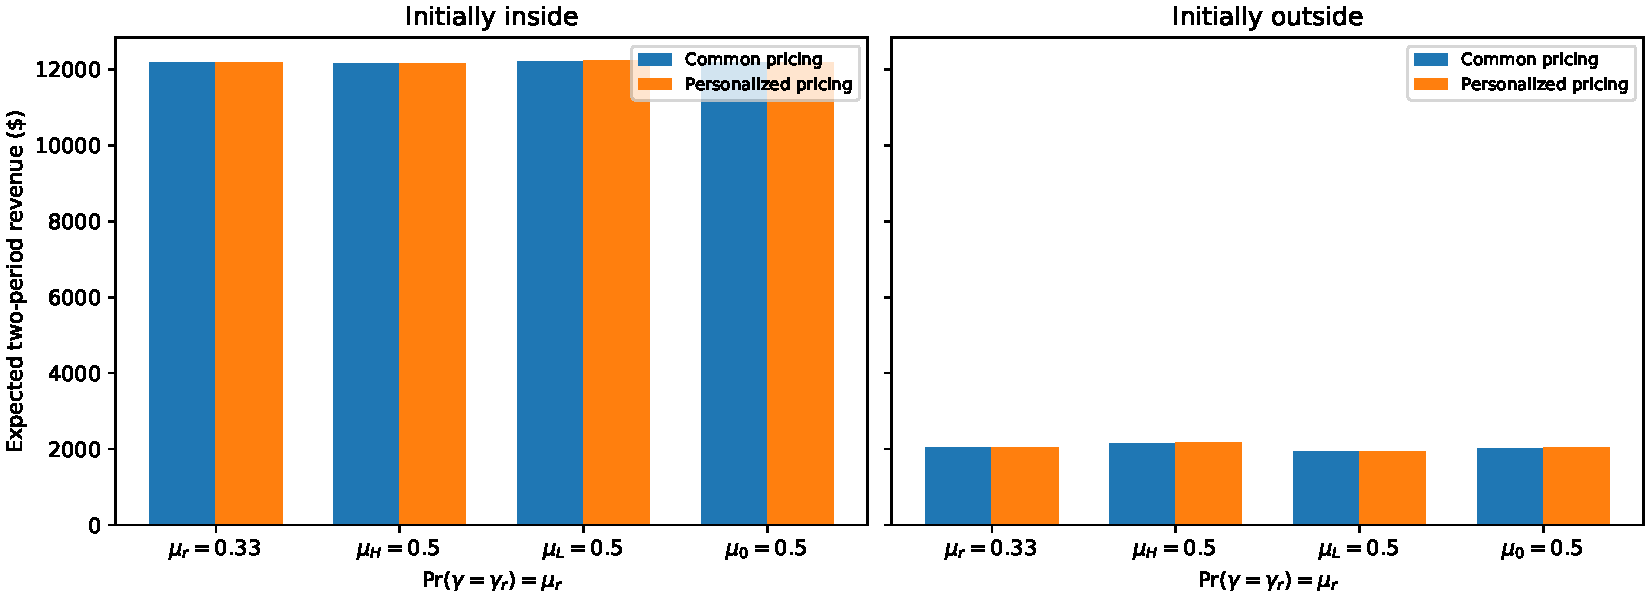
\includegraphics[width=.98\textwidth,height=.78\textheight,keepaspectratio]{assets/pricing/plain/information_friction_profits.pdf}
\end{frame}

% Original numbered slide 47
\gdef\shortbuttons{}
\begin{frame}[label=short-47]{Plain: Personalized vs Common Pricing}
\centering
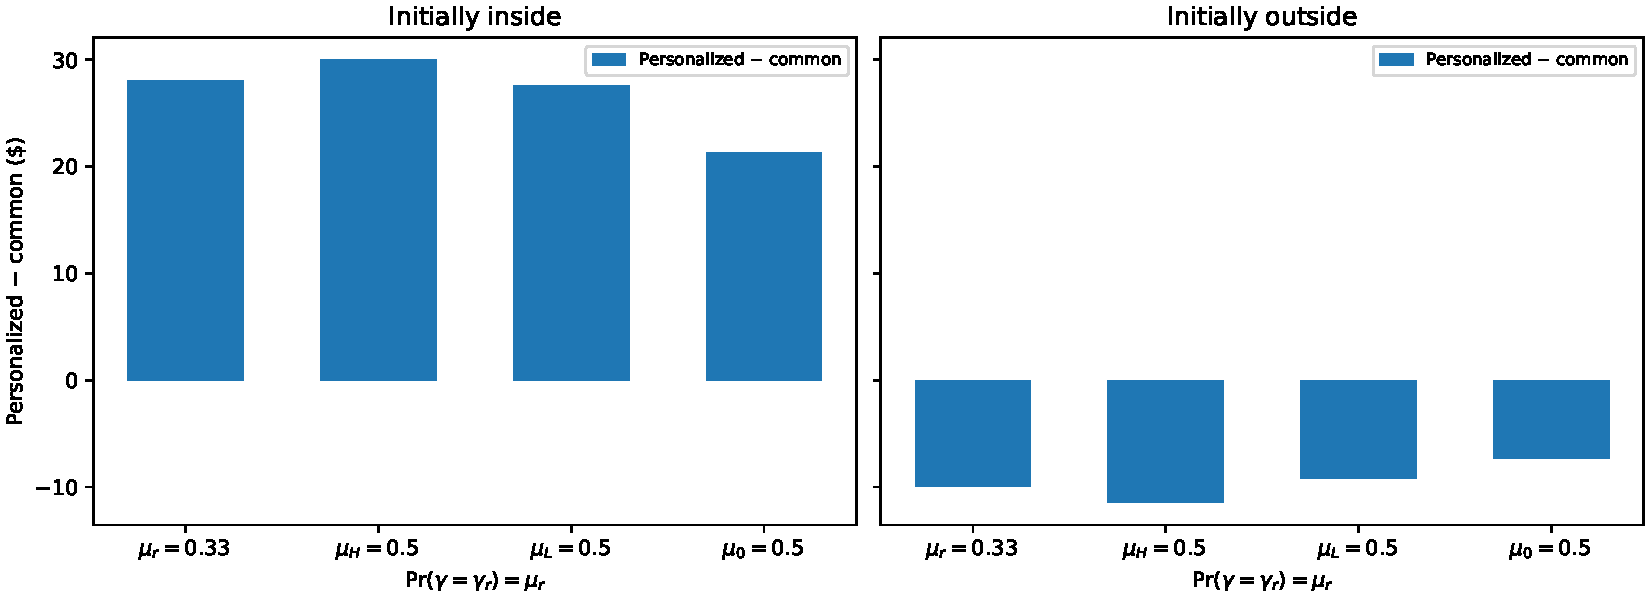
\includegraphics[width=.98\textwidth,height=.78\textheight,keepaspectratio]{assets/pricing/plain/information_friction_information_value.pdf}
\end{frame}

% Original numbered slide 57
\gdef\shortbuttons{}
\begin{frame}[label=short-57]{Plain: Price Paths under Type Uncertainty ($p_1$ to $p_2$)}
\centering
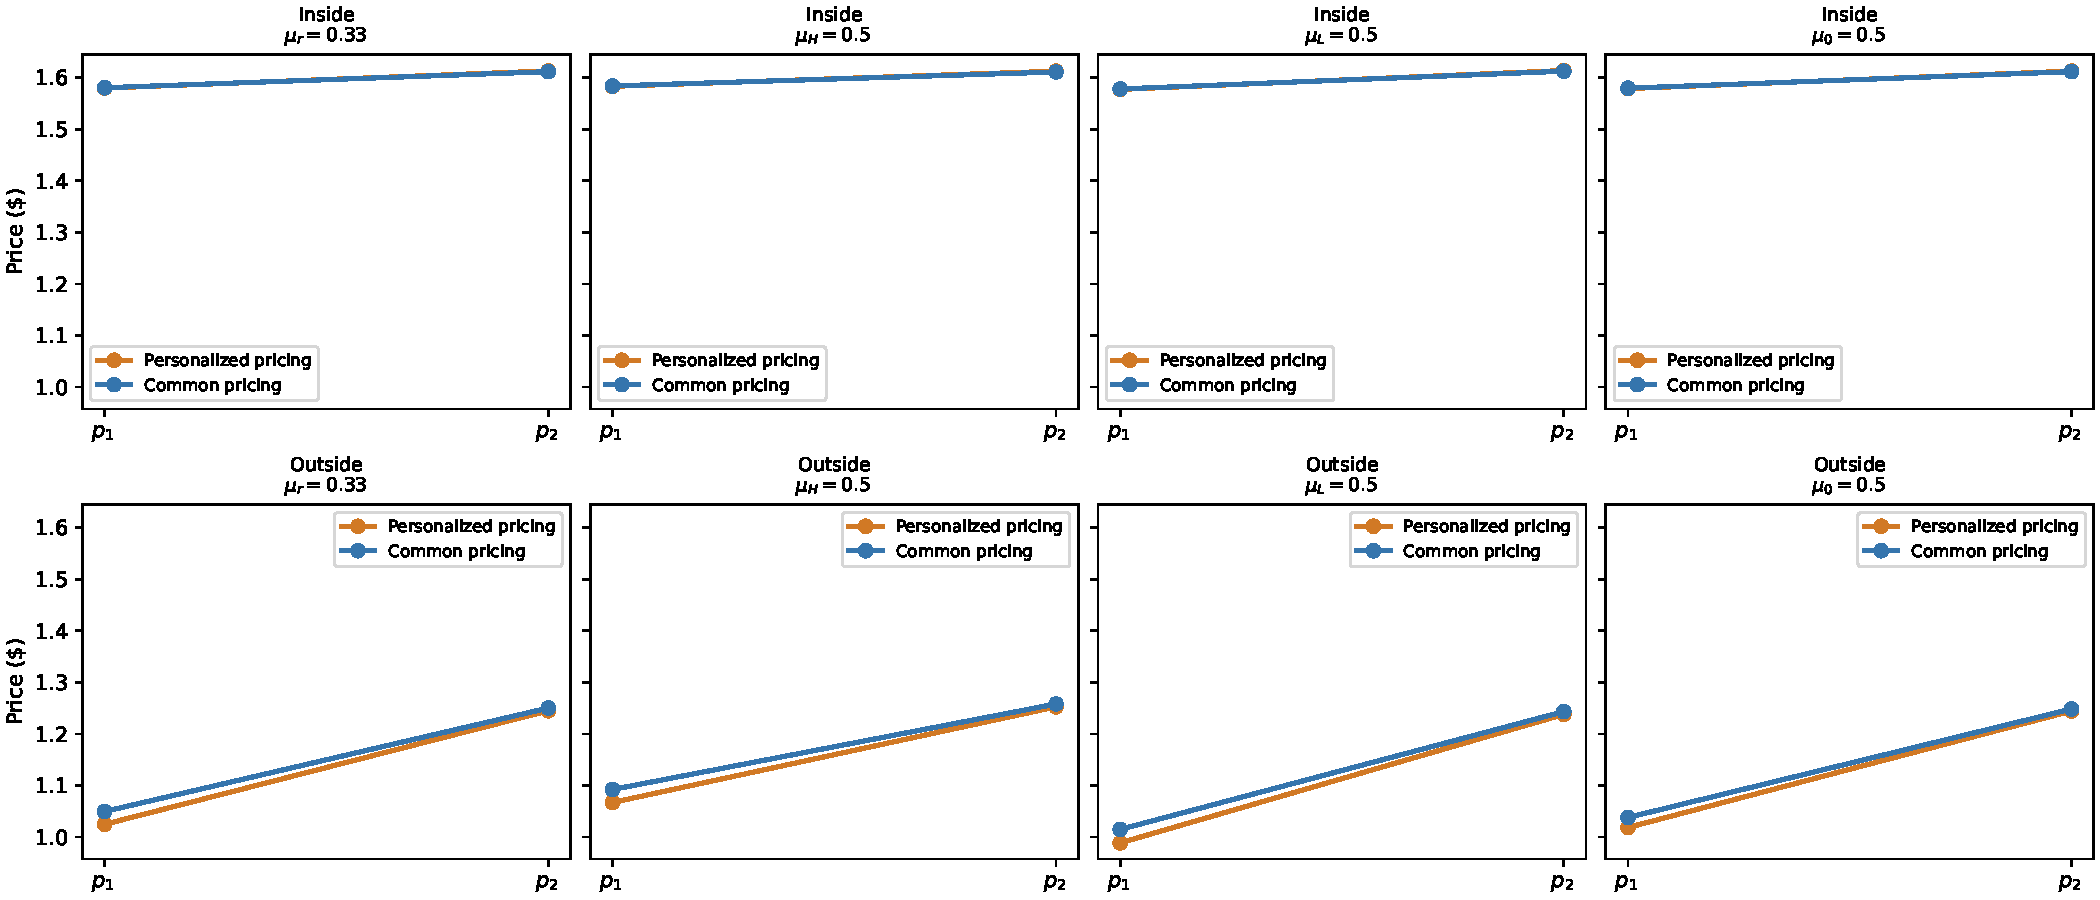
\includegraphics[width=.98\textwidth,height=.78\textheight,keepaspectratio]{assets/pricing/plain/information_friction_price_paths.pdf}
\end{frame}

% Original numbered slide 48
\gdef\shortbuttons{}
\begin{frame}[label=short-48]{Berry: Revenue under Type Uncertainty}
\centering
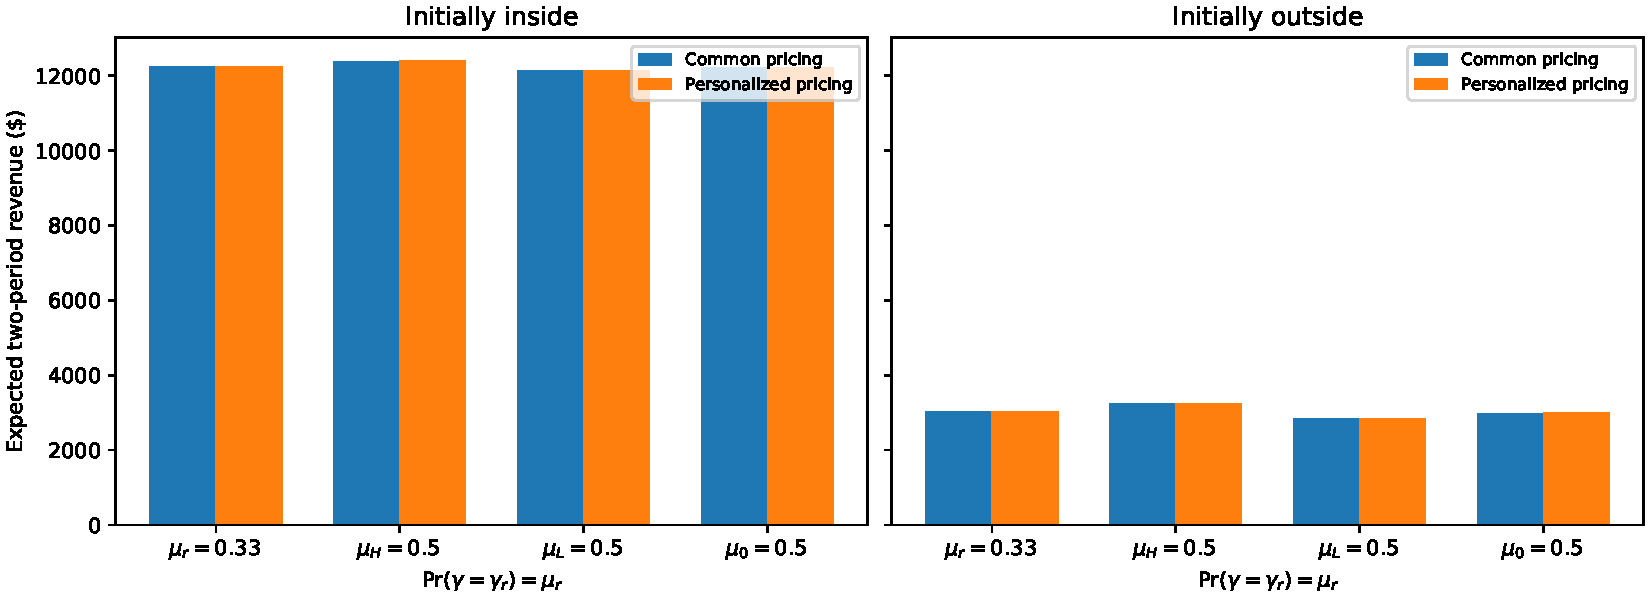
\includegraphics[width=.98\textwidth,height=.78\textheight,keepaspectratio]{assets/pricing/berry/information_friction_profits.pdf}
\end{frame}

% Original numbered slide 49
\gdef\shortbuttons{}
\begin{frame}[label=short-49]{Berry: Personalized vs Common Pricing}
\centering
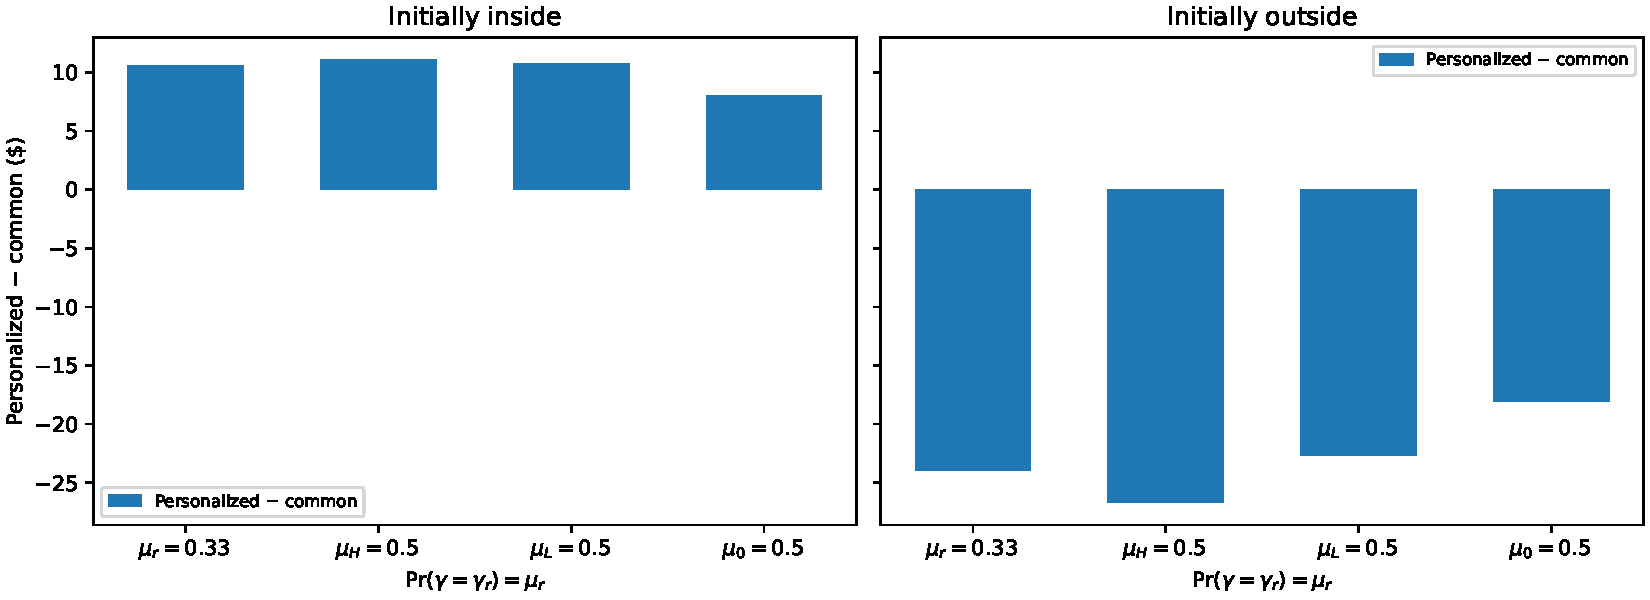
\includegraphics[width=.98\textwidth,height=.78\textheight,keepaspectratio]{assets/pricing/berry/information_friction_information_value.pdf}
\end{frame}

% Original numbered slide 59
\gdef\shortbuttons{}
\begin{frame}[label=short-59]{Berry: Price Paths under Type Uncertainty ($p_1$ to $p_2$)}
\centering
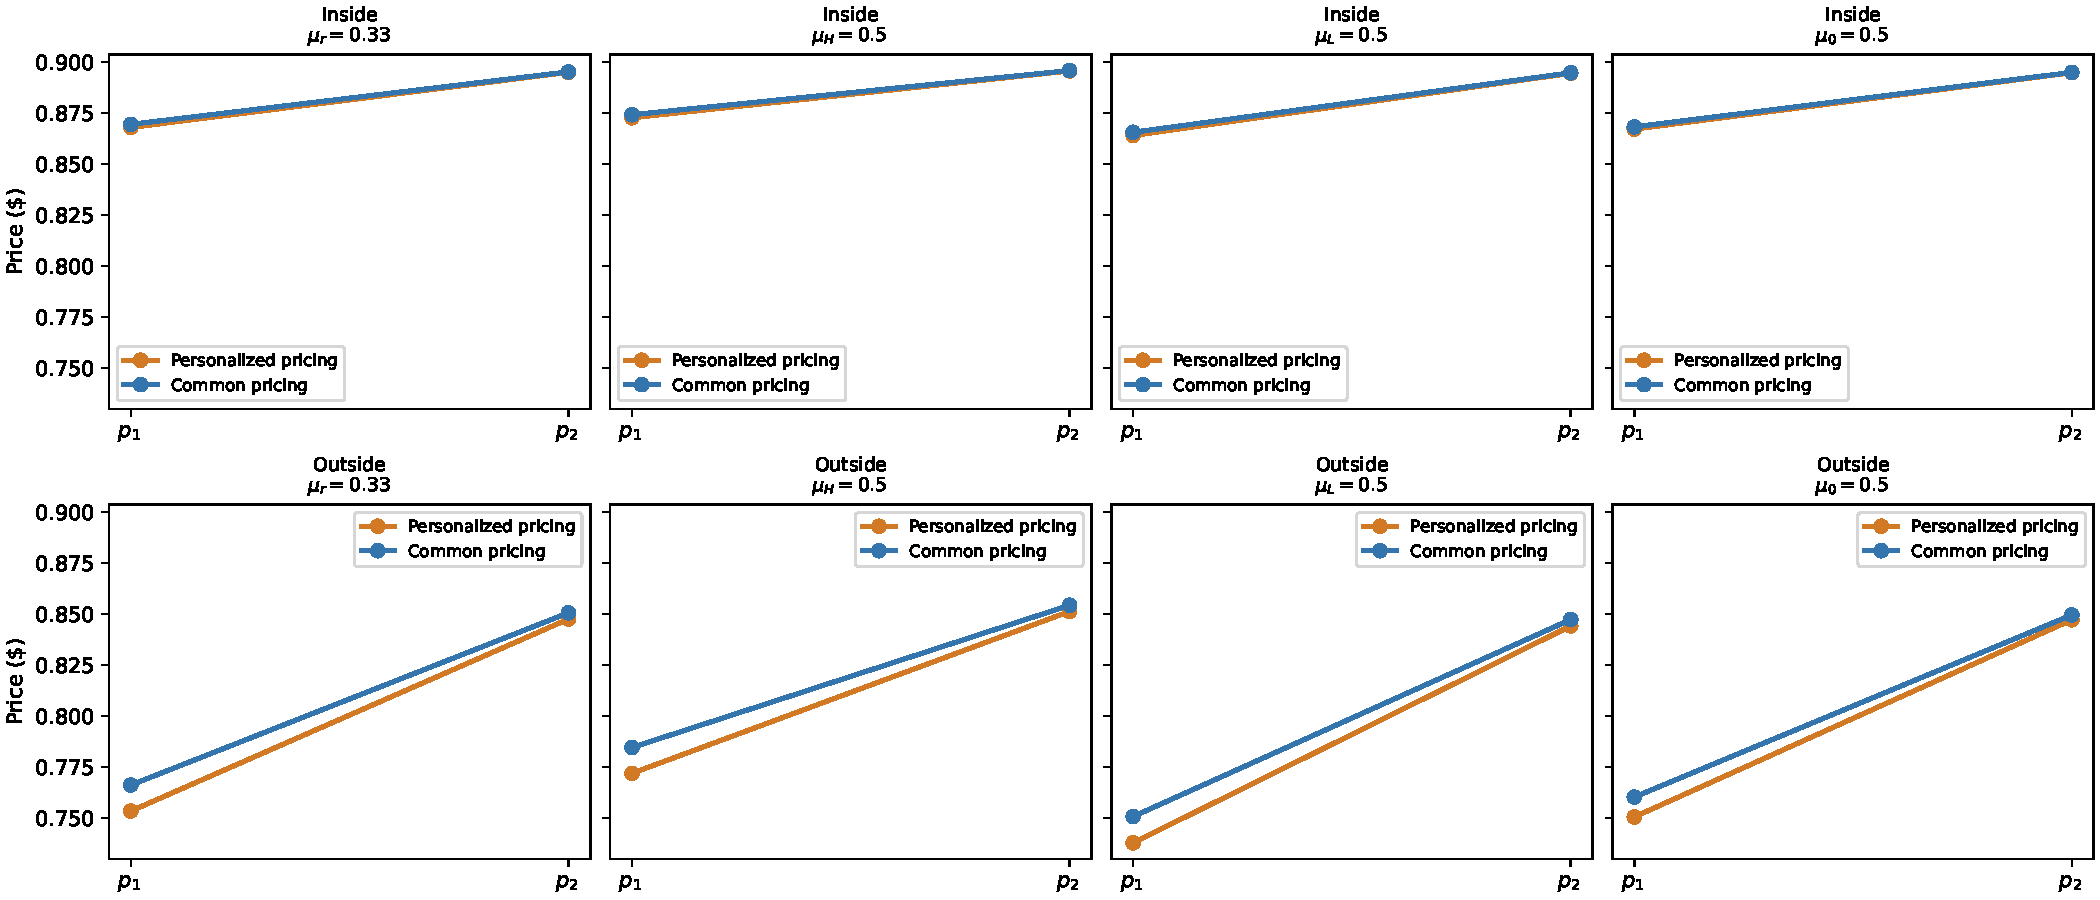
\includegraphics[width=.98\textwidth,height=.78\textheight,keepaspectratio]{assets/pricing/berry/information_friction_price_paths.pdf}
\end{frame}

\section{Conclusion}

% Original numbered slide 50
\gdef\shortbuttons{}
\begin{frame}[label=short-50]{Conclusion}
  \begin{itemize}
    \item Personalized pricing increases simulated revenue by up to $9.48\%$ relative to common pricing
    \item Consumers experience disutility from switching, needing to be subsidized $\approx\$1.75$ to switch products 
    \item Consumers enjoy habit and would be willing to pay $\$0.083$ to contribute another unit to the product's share of purchase history
  \end{itemize}
\end{frame}


% Original numbered slide 51
\gdef\shortbuttons{}
\begin{frame}[label=short-51]{Next Steps}
  \begin{itemize}
    \item Add firm learning to supply side
    \item Extend market structure on supply
    \item Add more product attributes to empirical estimation
    \item Estimate unobserved quality in BLP fashion
  \end{itemize}
\end{frame}


\appendix

\shortappendixtrue

\section{Appendix}

% Original numbered slide 22
\gdef\shortbuttons{\hyperlink{short-21}{\beamergotobutton{Back to Data Sources}}}
\begin{frame}[label=short-22,noframenumbering]{Sample Statistics: Purchase Activity}
  \centering
  \small
  \renewcommand{\arraystretch}{1.15}
  \begin{tabular}{lrr}
    \toprule
     & Full sample & Yogurt sample \\
    \midrule
    Households & 37,827 & 15,106 \\
    Observed panel years & 3.96 & 3.16 \\
    Trips per household & 493.13 & 20.26 \\
    Trips per observed week (approx.) & 2.27 & 0.11 \\
    Distinct UPCs per household & 1,178.31 & 13.89 \\
    Purchase lines per household & 3,397.64 & 45.15 \\
    Packages per household & 4,669.07 & 93.77 \\
    \bottomrule
  \end{tabular}

  \medskip
  {\footnotesize All statistics except household counts are means.}
\end{frame}





% Original numbered slide 5
\gdef\shortbuttons{\hyperlink{short-4}{\beamergotobutton{Back to HHI}}}
\begin{frame}[label=short-5,noframenumbering]{Flavor Popularity}
  \centering
    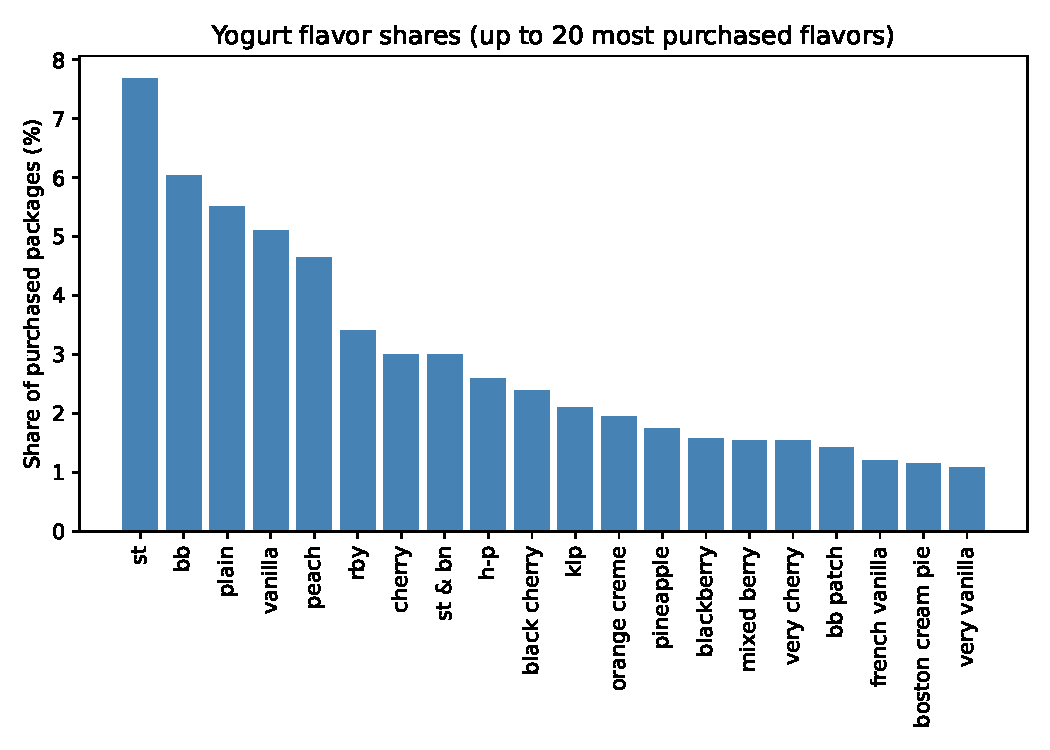
\includegraphics[width=.95\textwidth,height=.74\textheight,keepaspectratio]{../writeup/1108_writeup/assets/results/summary_statistics/flavor_shares.pdf}
\end{frame}


% Original numbered slide 9
\gdef\shortbuttons{\hyperlink{short-10}{\beamergotobutton{Back to First Period Optimization}}}
\begin{frame}[label=short-9,noframenumbering]{Optimal Terminal Price and Profit}
  \begin{tcolorbox}
    [
    boxsep=0pt,
    left=2pt, right=2pt,
    top=1pt, bottom=1pt,
    before skip=2pt, after skip=2pt
    ]
    \setlength{\abovedisplayskip}{2pt}
    \setlength{\belowdisplayskip}{2pt}
    \begin{align*}
      \frac{\partial\pi_2(h_1)}{\partial p_2(h_1)} &= s_2(h_1) + (p_2 - c)\frac{\partial s_2(h_1)}{\partial p_2(h_1)} \\
      p_2^*(h_1)&= c + \frac{1}{\alpha(1-s_2^*(h_1))} \\
      \pi^*_2(p_2^*(h_1); h_1) &= \frac{s_2^*(h_1)}{\alpha(1-s_2^*(h_1))}
    \end{align*}
  \end{tcolorbox}
  \begin{itemize}
    \item Optimal period two price is cost plus a demand markup term
    \item Period two profit at optimal prices is the odds of purchase, scaled by the inverse price sensitivity
  \end{itemize}
\end{frame}


% Original numbered slide 11
\gdef\shortbuttons{\hyperlink{short-10}{\beamergotobutton{Back to First Period Optimization}}}
\begin{frame}[label=short-11,noframenumbering]{Optimal Profit Given Switching Type}
  \begin{tcolorbox}
    [
    boxsep=0pt,
    left=2pt, right=2pt,
    top=1pt, bottom=1pt,
    before skip=2pt, after skip=2pt
    ]
    \setlength{\abovedisplayskip}{2pt}
    \setlength{\belowdisplayskip}{2pt}
    \begin{align*}
      \frac{d\Pi}{d\gamma} &= \frac{q(h)s_1^*(h) - \delta s_1^*(h)s_2^*(j) + \delta(1-s_1^*(h))s_2^*(0)}{\alpha}
    \end{align*}
  \end{tcolorbox}
  \begin{itemize}
    \item There are two interpretations:
    \begin{enumerate}
      \item If $h_0=j$, $q(h)<0$, leading us to ambiguous signage as we raise profits from initially outside consumers but see opposing forces for the initially inside: leave in period one, return in period two 
      \item If $h_0=0$, $q(h)>0\Rightarrow \frac{d\Pi}{d\gamma} > 0$, meaning that profits increase as $\gamma$ increases
    \end{enumerate}
    \item Points to firms potentially reaping great benefit from knowing consumer types and histories
  \end{itemize}
\end{frame}


% Original numbered slide 52
\gdef\shortbuttons{\hyperlink{short-10}{\beamergotobutton{Back to First Period Optimization}}}
\begin{frame}[label=short-52,noframenumbering]{Shares and Elasticities}
  \begin{tcolorbox}
    [
    boxsep=0pt,
    left=2pt, right=2pt,
    top=1pt, bottom=1pt,
    before skip=2pt, after skip=2pt
    ]
    \setlength{\abovedisplayskip}{2pt}
    \setlength{\belowdisplayskip}{2pt}
    \begin{gather*}
      s_t(h) = \frac{e^{v_t(h)}}{1+e^{v_t(h)}}, \ s_{0t}(h) = 1-s_t(h) \\
      \frac{\partial s_t(h)}{\partial p_t(h)} = -\alpha s_t(h)(1-s_t(h)) \\
      \frac{\partial s_t(h)}{\partial\gamma} = q(h)s_t(h)(1-s_t(h))
    \end{gather*}
  \end{tcolorbox}
  \end{frame}


% Original numbered slide 12
\gdef\shortbuttons{\hyperlink{short-14}{\beamergotobutton{Back to Optimal Prices}}}
\begin{frame}[label=short-12,noframenumbering]{Pricing Simulations Specification}
  \centering
  \small
  \begin{tabular}{lll}
    \toprule
    Parameter & Description & Value \\
    \midrule
    $\beta$ & Inside-good intercept & $2$ \\
    $\alpha$ & Price sensitivity & $1$ \\
    $\delta$ & Discount factor (no discounting) & $1$ \\
    $c$ & Marginal cost & $0$ \\
    $\gamma$ & Switching preference & $[-3,3]$ \\
    \midrule
    \multicolumn{2}{l}{Initial Consumption State}
      & $h_0\in\{0,j\}$ \\
    \multicolumn{2}{l}{Feasible Prices}
      & $p_t(h)\in\mathbb{R}$ \\
    \bottomrule
  \end{tabular}
  \begin{itemize}
    \item Allow for negative pricing
    \item Firm has knowledge of both type and history, allowing for targeted pricing
    \item Four consumption histories possible $(h_0, h_1) \in \{(0,0), (0,j), (j,j), (j,0)\}$
  \end{itemize}
\end{frame}


% Original numbered slide 13
\gdef\shortbuttons{\hyperlink{short-14}{\beamergotobutton{Back to Optimal Prices}}}
\begin{frame}[label=short-13,noframenumbering]{Results}
  \begin{center}\small\begin{tabular}{crrrrrr}\toprule
  $x_0$ & $\gamma$ & $p_1^*$ & $p_2^*(j)$ & $p_2^*(0)$ & $\Pi^*$ & $\Pi^{*\prime}$\\\midrule
  $j$ & -3 & 3.358 & 3.926 & 1.120 & 5.284 & -1.445\\
  $j$ & -1 & 2.211 & 2.557 & 1.567 & 2.768 & -0.993\\
  $j$ & 0 & 2.000 & 2.000 & 2.000 & 2.000 & -0.500\\
  $j$ & 1 & 2.271 & 1.567 & 2.557 & 1.838 & 0.177\\
  $j$ & 3 & 3.814 & 1.120 & 3.926 & 2.934 & 0.730\\
  $0$ & -3 & -0.901 & 3.926 & 1.120 & 1.026 & 0.177\\
  $0$ & -1 & 1.005 & 2.557 & 1.567 & 1.562 & 0.376\\
  $0$ & 0 & 2.000 & 2.000 & 2.000 & 2.000 & 0.500\\
  $0$ & 1 & 2.995 & 1.567 & 2.557 & 2.562 & 0.624\\
  $0$ & 3 & 4.905 & 1.120 & 3.926 & 4.025 & 0.823\\
  \bottomrule\end{tabular}\end{center}
\end{frame}


% Original numbered slide 15
\gdef\shortbuttons{\hyperlink{short-14}{\beamergotobutton{Back to Optimal Prices}}}
\begin{frame}[label=short-15,noframenumbering]{Optimal Profit}
  \centering
  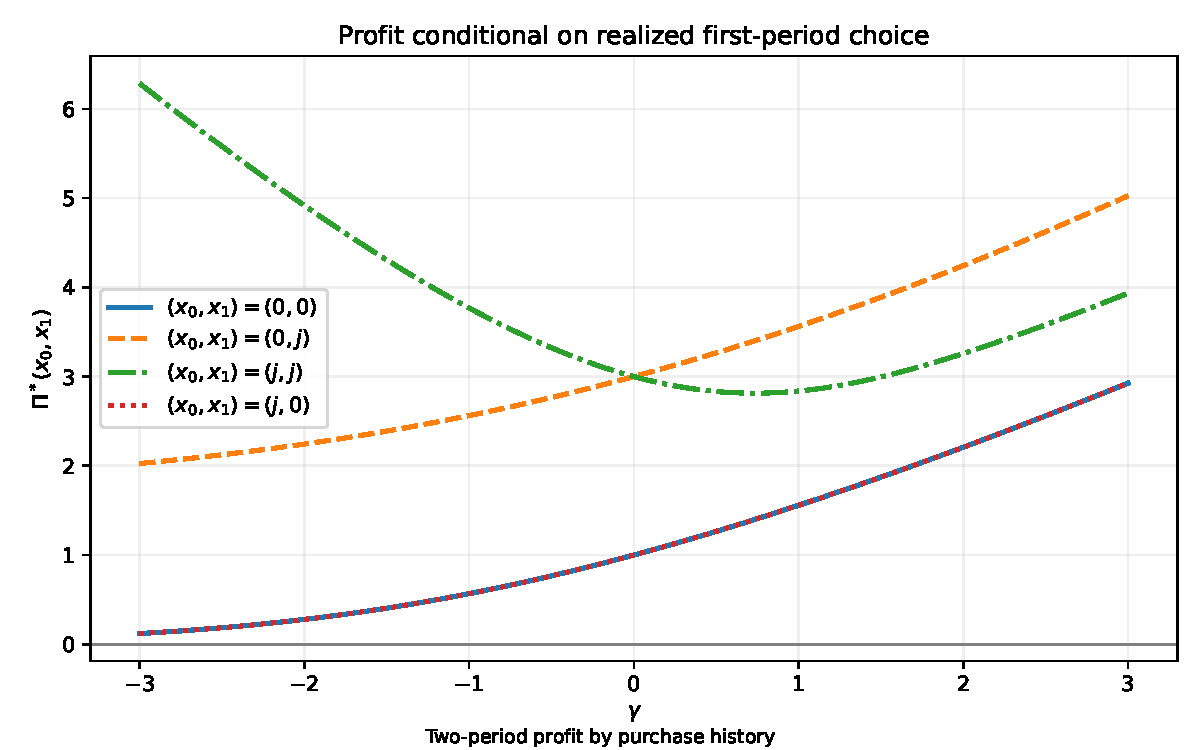
\includegraphics[width=.75\textwidth,height=.68\textheight,keepaspectratio]{assets/theory_delta1/all_state_realized_profit.pdf}
\end{frame}


% Original numbered slide 16
\gdef\shortbuttons{\hyperlink{short-14}{\beamergotobutton{Back to Optimal Prices}}}
\begin{frame}[label=short-16,noframenumbering]{Optimal Price Ratio}
  \centering
  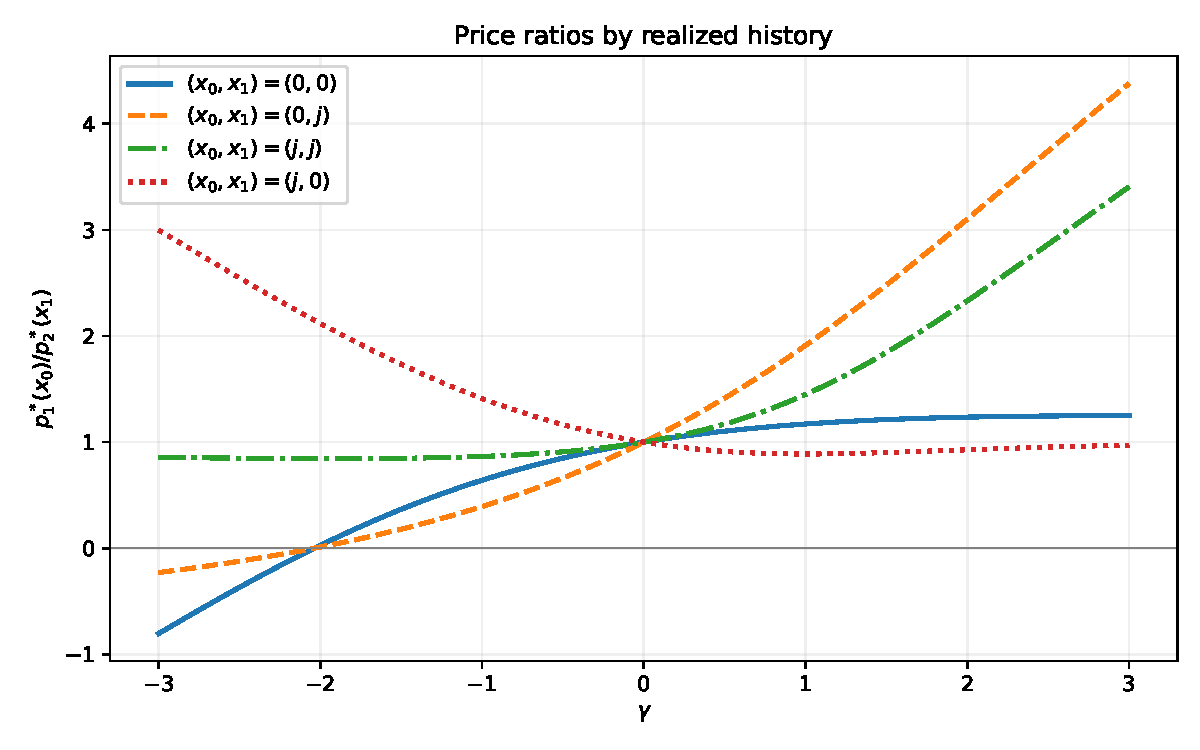
\includegraphics[width=.75\textwidth,height=.68\textheight,keepaspectratio]{assets/theory_delta1/all_state_price_ratios.pdf}
\end{frame}


% Original numbered slide 17
\gdef\shortbuttons{\hyperlink{short-14}{\beamergotobutton{Back to Optimal Prices}}}
\begin{frame}[label=short-17,noframenumbering]{Discussion}
  \begin{itemize}
    \item Two mechanisms: Induce and harvest, Retain and gain
    \item Most profit from those who are habitual inside purchasers 
    \item Least profit from those who purchase outside in period 1 across all levels of gamma
    \item Interesting when $(j,j)$ and $(0,0)$ cross
  \end{itemize}
\end{frame}


% Original numbered slide 19
\gdef\shortbuttons{\hyperlink{short-20}{\beamergotobutton{Back to Personalized vs Common Pricing}}}
\begin{frame}[label=short-19,noframenumbering]{Known versus Uncertain Switching Type}
\centering
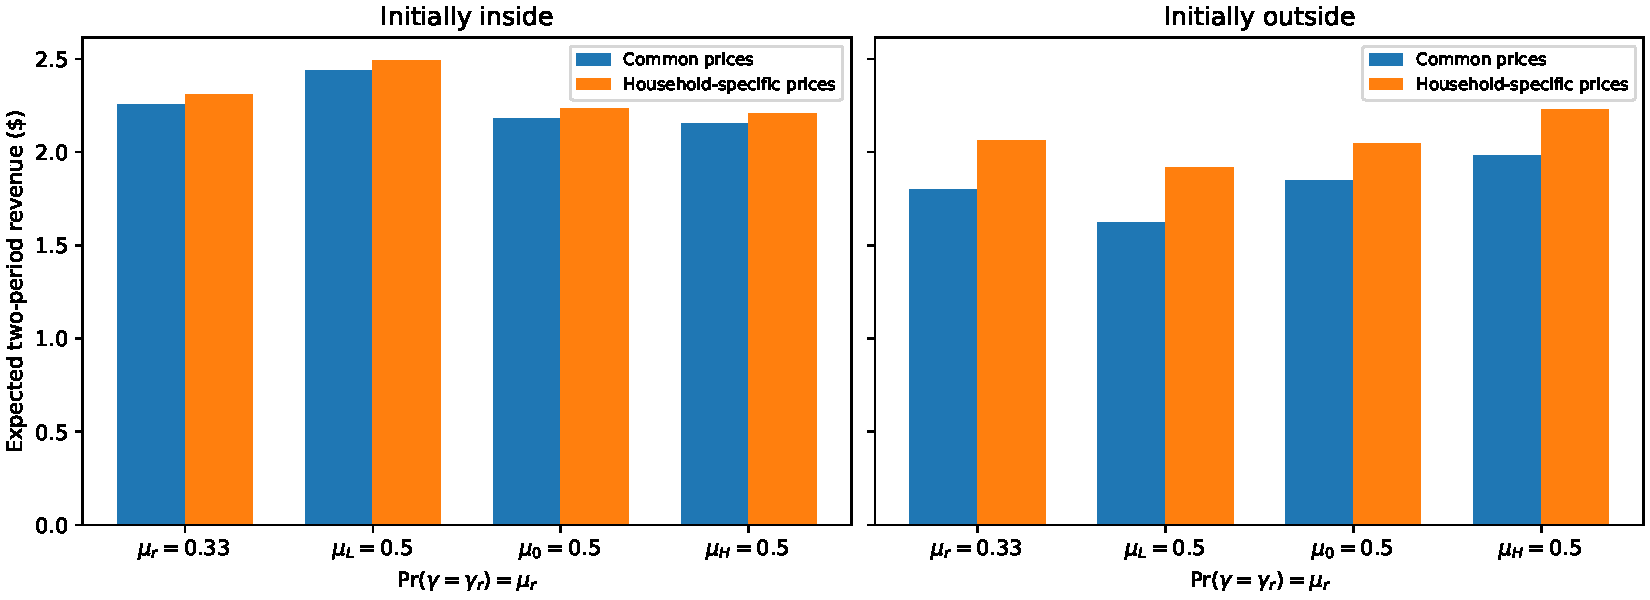
\includegraphics[width=.98\textwidth,height=.78\textheight,keepaspectratio]{assets/theory_delta1/gamma_uncertainty/profits.pdf}
\end{frame}


% Original numbered slide 53
\gdef\shortbuttons{\hyperlink{short-20}{\beamergotobutton{Back to Personalized vs Common Pricing}}}
\begin{frame}[label=short-53,noframenumbering]{Type Uncertainty: Price Paths}
\centering
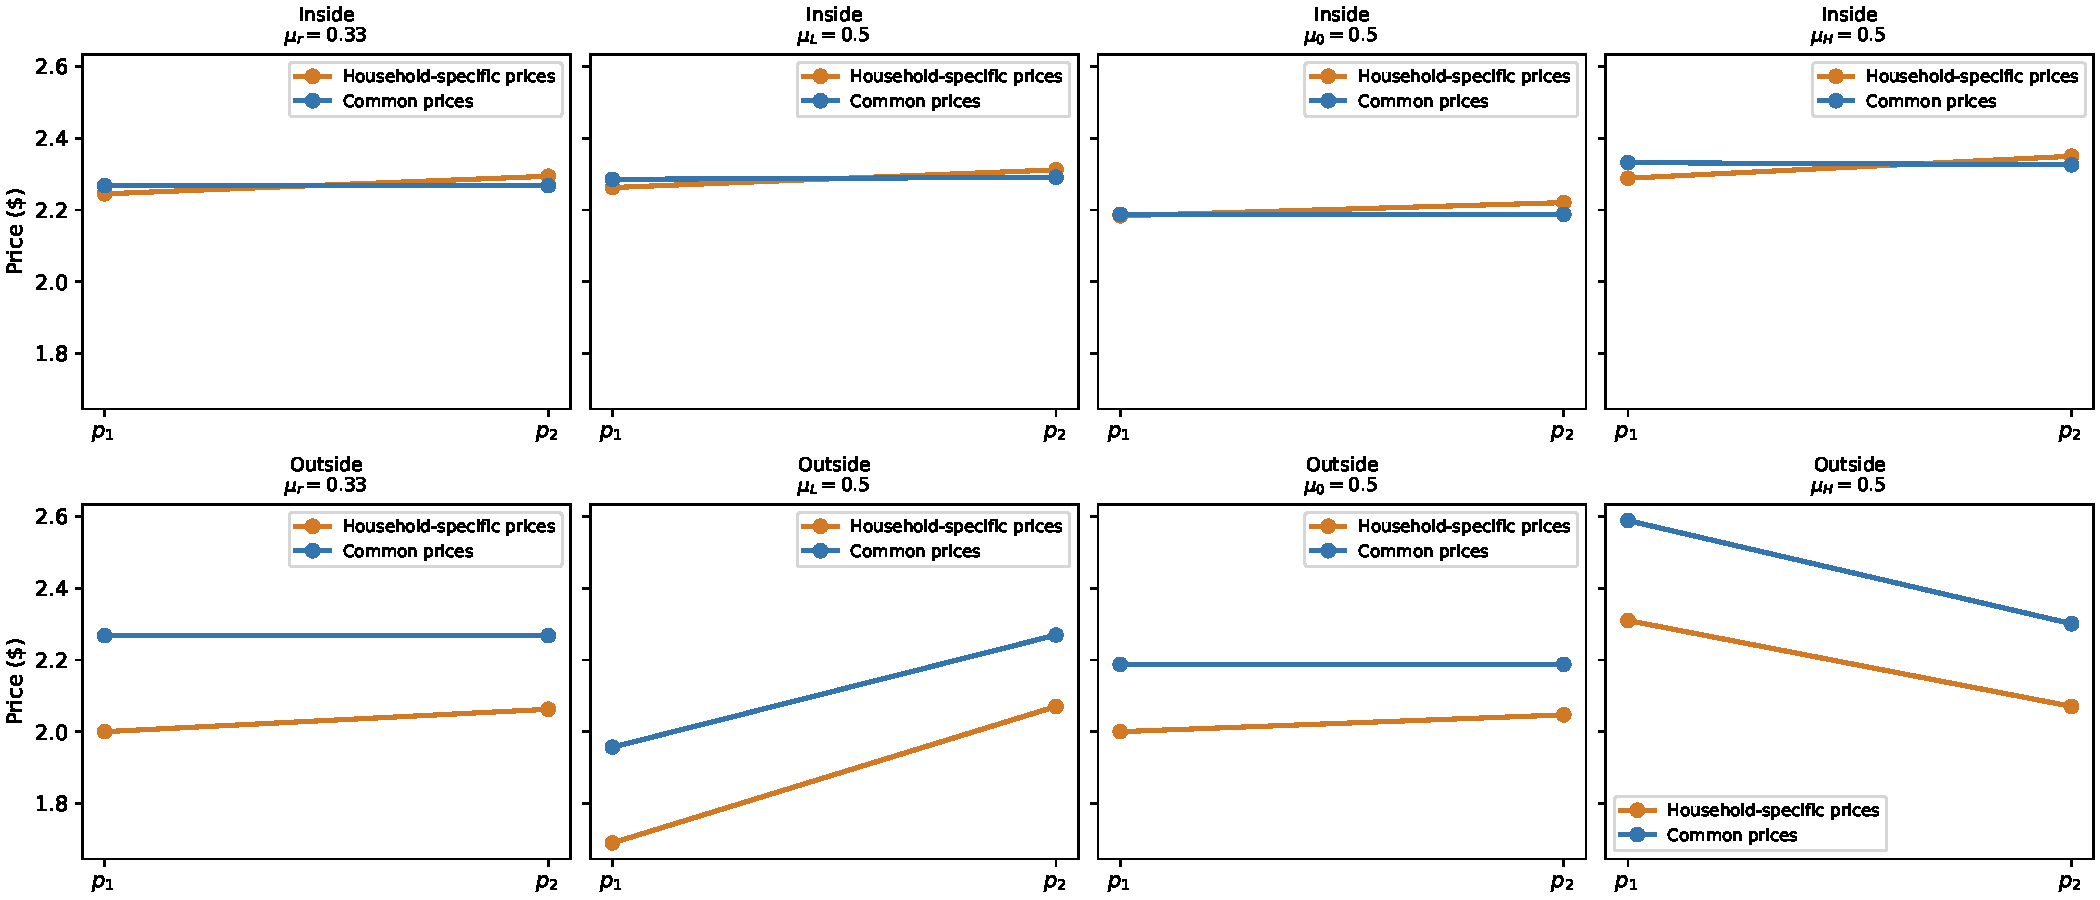
\includegraphics[width=.98\textwidth,height=.78\textheight,keepaspectratio]{assets/theory_delta1/gamma_uncertainty/first_prices.pdf}
\end{frame}


% Original numbered slide 54
\gdef\shortbuttons{\hyperlink{short-20}{\beamergotobutton{Back to Personalized vs Common Pricing}}}
\begin{frame}[label=short-54,noframenumbering]{Type Uncertainty: Price Paths}
\centering
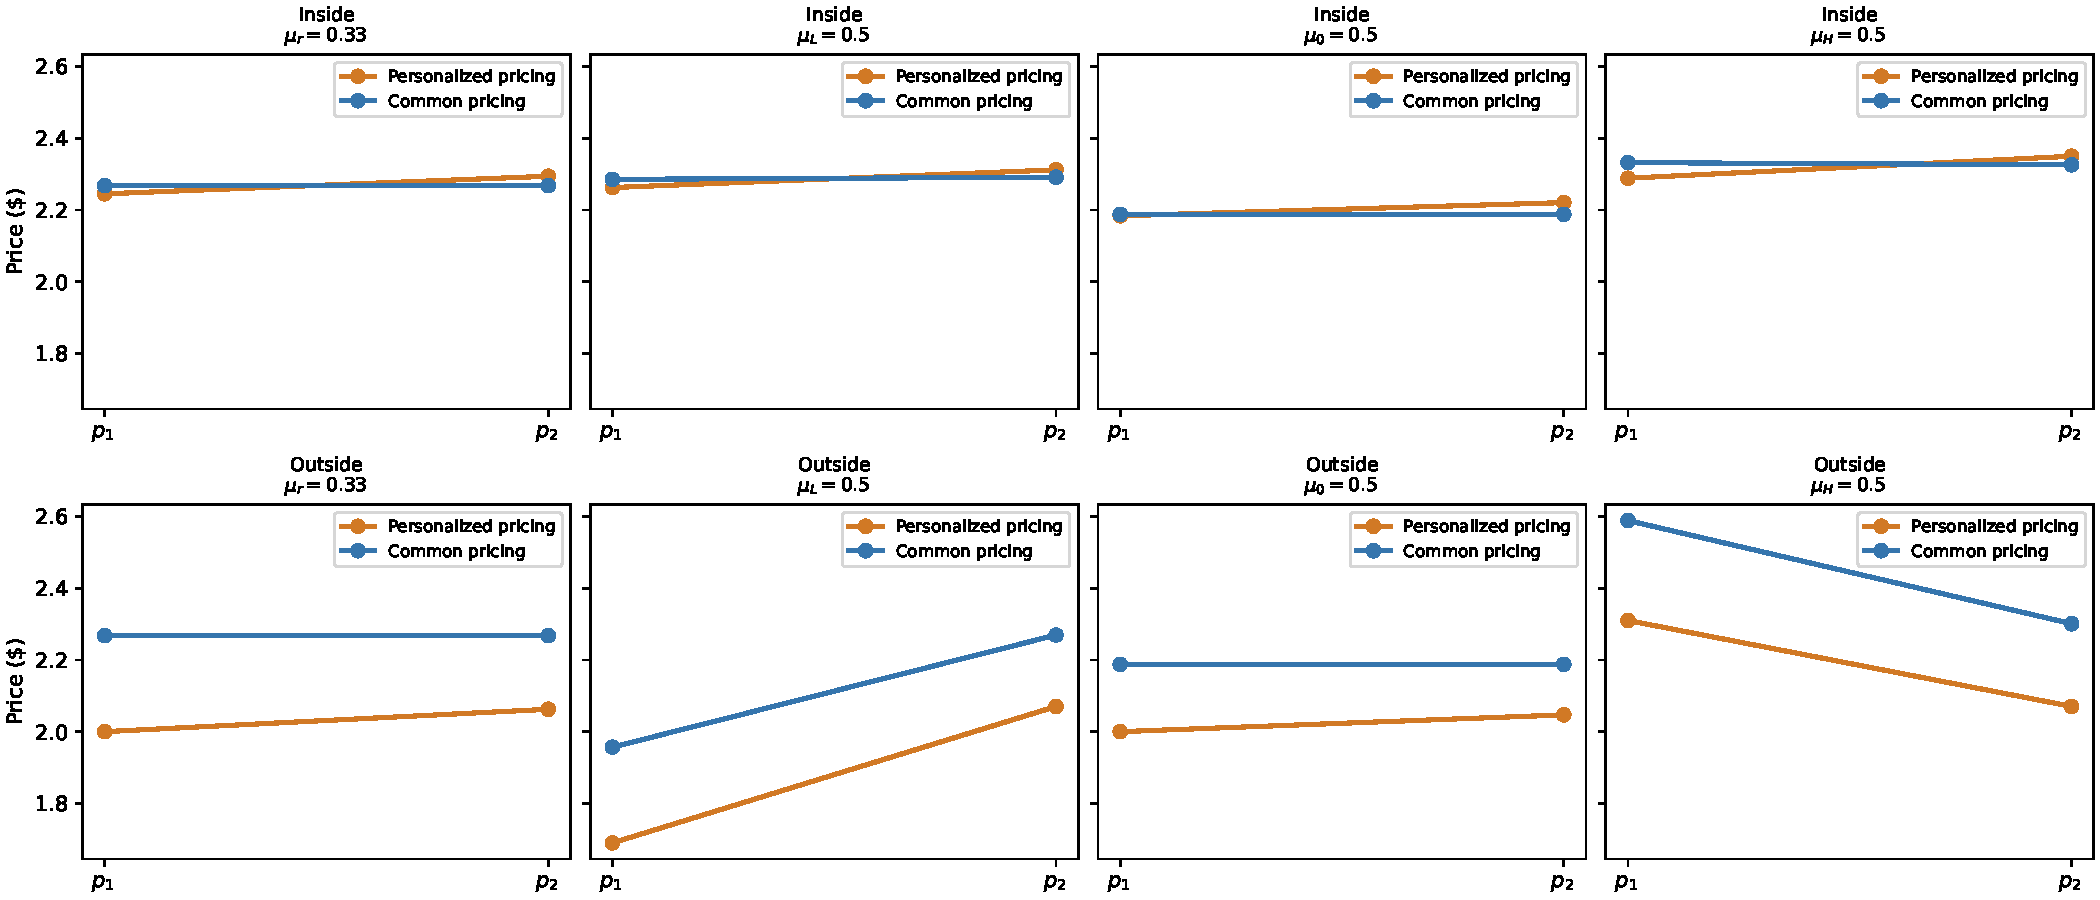
\includegraphics[width=.98\textwidth,height=.78\textheight,keepaspectratio]{assets/theory_delta1/gamma_uncertainty/terminal_prices.pdf}
\end{frame}


% Original numbered slide 28
\gdef\shortbuttons{\hyperlink{short-29}{\beamergotobutton{Back to Estimation}}}
\begin{frame}[label=short-28,noframenumbering]{Probability and Shares}
  \begin{align*}
    P_{ijt} &= \frac{\text{exp}\{V_{ijt}\}}{1 + \sum_{k\in J}\text{exp}\{V_{ikt}\}} \\
    &\text{s.t.} \ V_{ijt} = U_{ijt} - \varepsilon_{ijt} \\
    s_{jt} &= \frac{1}{N}\sum_{n=1}^{N}P_{ijt}
  \end{align*}
  \begin{itemize}
    \item Use deterministic utility to form purchase probabilities
    \item Take average probability for product $j$ across individuals $i\in N$ to recover shares 
  \end{itemize}
\end{frame}


% Original numbered slide 55
\gdef\shortbuttons{\hyperlink{short-29}{\beamergotobutton{Back to Estimation}}}
\begin{frame}[label=short-55,noframenumbering]{Demand: Price-Control Comparison}
\begin{table}[htbp]\centering\small
\caption{Demand estimates with and without price controls; standard errors in parentheses}
\label{tab:demand-comparison}
\begin{adjustbox}{max width=\linewidth}
\begin{tabular}{lrr}\toprule
Parameter & No controls & With controls\\\midrule
Mean novelty & -0.7732 (0.0095) & -0.7861 (0.0091) \\
Mean habit & 0.0369 (0.0002) & 0.0373 (0.0002) \\
SD novelty & 0.8003 (0.0085) & 0.7999 (0.0082) \\
SD habit & 0.0783 (0.0004) & 0.0793 (0.0004) \\
\bottomrule\end{tabular}
\end{adjustbox}
\end{table}

\end{frame}


% Original numbered slide 56
\gdef\shortbuttons{\hyperlink{short-29}{\beamergotobutton{Back to Estimation}}}
\begin{frame}[label=short-56,noframenumbering]{Controlled Demand Estimates}
\begin{table}[htbp]\centering\small
\caption{Demand estimates with price controls}
\label{tab:demand-estimates-controlled}
\begin{adjustbox}{max width=\linewidth}
\begin{tabular}{lrr}\toprule
Parameter & Estimate & Standard error\\\midrule
Inside constant $\beta_0$ & 1.4762 & 0.0072 \\
Berry vs. other & -0.6556 & 0.0034 \\
Plain vs. other & -0.1192 & 0.0066 \\
Mean price coefficient $E[\alpha_i]$ & -1.0349 & 0.0051 \\
Mean novelty & -0.7861 & 0.0091 \\
Mean habit & 0.0373 & 0.0002 \\
SD price coefficient $\mathrm{SD}(\alpha_i)$ & 0.7957 & 0.0063 \\
SD novelty & 0.7999 & 0.0082 \\
SD habit & 0.0793 & 0.0004 \\
Price control $\rho$ & 0.1959 & 0.0047 \\
\bottomrule\end{tabular}
\end{adjustbox}
\end{table}

\end{frame}


% Original numbered slide 61
\gdef\shortbuttons{\hyperlink{short-29}{\beamergotobutton{Back to Estimation}}}
\begin{frame}[label=short-61,noframenumbering]{Controlled Fit: Price First Stages}
\begin{table}[htbp]\centering\small
\caption{Price first stages for the controlled specification}
\label{tab:updated-first-stage}
\begin{tabular}{lrrrr}\toprule
Flavor & IV slope & Cluster SE & $F$ & Partial $R^2$\\\midrule
Other & -34.680 & 0.966 & 1288.26 & 0.0213 \\
Berry & -33.105 & 1.377 & 578.20 & 0.0192 \\
Plain & -28.585 & 3.085 & 85.87 & 0.0076 \\
\bottomrule\end{tabular}
\end{table}

\end{frame}


% Original numbered slide 30
\gdef\shortbuttons{\hyperlink{short-32}{\beamergotobutton{Back to Distributions}}}
\begin{frame}[label=short-30,noframenumbering]{Estimates}
  \centering
  \begin{table}[htbp]\centering\small
\caption{Demand estimates without price controls}
\label{tab:demand-estimates}
\begin{adjustbox}{max width=\linewidth}
\begin{tabular}{lrr}\toprule
Parameter & Estimate & Standard error\\\midrule
Inside constant $\beta_0$ & 1.2173 & 0.0035 \\
Berry vs. other & -0.6241 & 0.0034 \\
Plain vs. other & -0.2719 & 0.0054 \\
Mean price coefficient $E[\alpha_i]$ & -0.8940 & 0.0044 \\
Mean novelty & -0.7732 & 0.0095 \\
Mean habit & 0.0369 & 0.0002 \\
SD price coefficient $\mathrm{SD}(\alpha_i)$ & 0.9019 & 0.0099 \\
SD novelty & 0.8003 & 0.0085 \\
SD habit & 0.0783 & 0.0004 \\
\bottomrule\end{tabular}
\end{adjustbox}
\end{table}

\end{frame}


% Original numbered slide 33
\gdef\shortbuttons{\hyperlink{short-32}{\beamergotobutton{Back to Distributions}}}
\begin{frame}[label=short-33,noframenumbering]{Discussion}
  \begin{itemize}
    \item Mean novelty effect is equivalent to $\approx\$1.75$ increase 
    \item Habit provides some utility
    \item Both plain and berry are less preferred than other flavors
  \end{itemize}
  \begin{tcolorbox}
    How can the firm use the distribution of switching types to price discriminate?
  \end{tcolorbox}
\end{frame}


% Original numbered slide 62
\gdef\shortbuttons{\hyperlink{short-31}{\beamergotobutton{Back to Implied Willingness to Pay}}}
\begin{frame}[label=short-62,noframenumbering]{Controlled Fit: Willingness to Pay}
\begin{table}[htbp]\centering\small
\caption{Implied willingness to pay with price controls}
\label{tab:wtp-demand_controlled}
\begin{adjustbox}{max width=\linewidth}
\begin{tabular}{lrr}\toprule
Utility term & Mean WTP & Population SD\\\midrule
Inside constant $\beta_0$ & 2.2696 & 1.7451 \\
Berry vs. other & -1.0081 & 0.7751 \\
Plain vs. other & -0.1832 & 0.1409 \\
novelty & -1.2086 & 1.8083 \\
own stock & 0.0574 & 0.1600 \\
\bottomrule\end{tabular}
\end{adjustbox}
\end{table}

\end{frame}


% Original numbered slide 36
\gdef\shortbuttons{\hyperlink{short-44}{\beamergotobutton{Back to Comparison}}}
\begin{frame}[label=short-36,noframenumbering]{Results: Berry Inside}
  \centering
  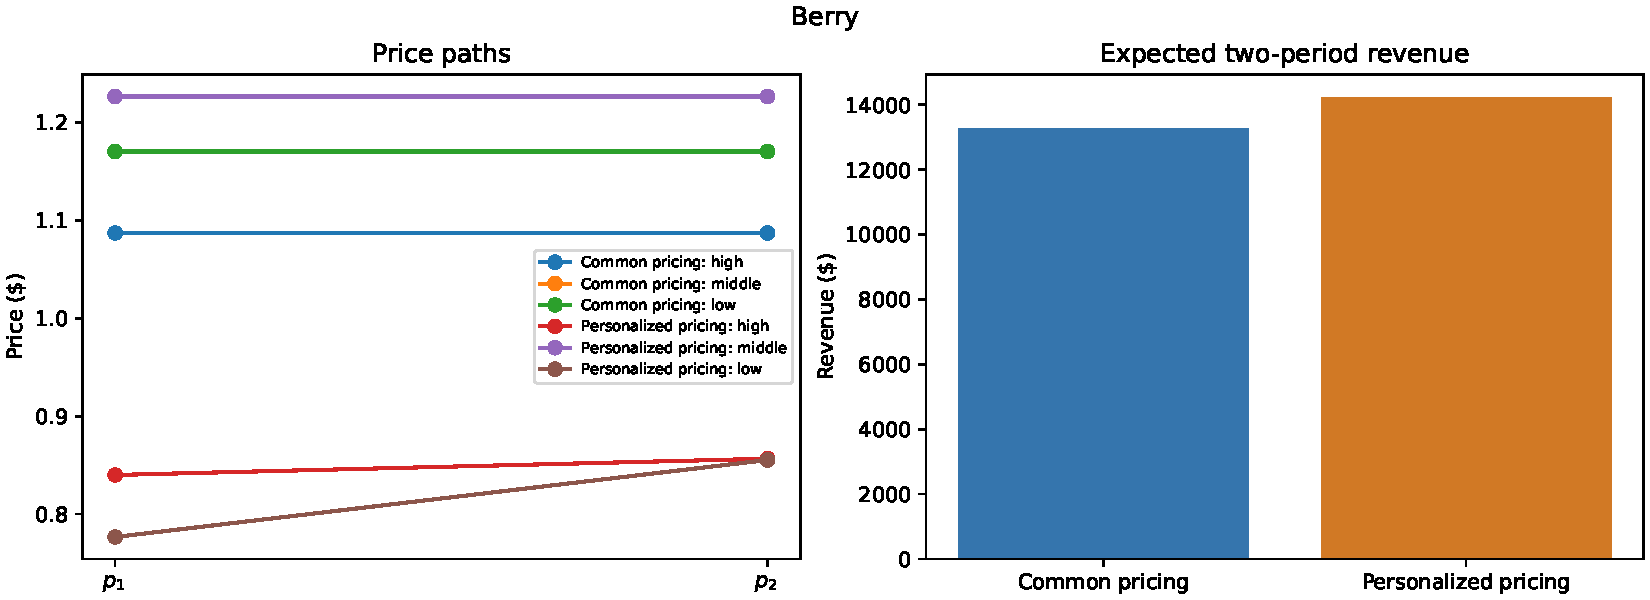
\includegraphics[width=\textwidth]{assets/pricing/berry/household_coupon_results.pdf}
\end{frame}


% Original numbered slide 37
\gdef\shortbuttons{\hyperlink{short-44}{\beamergotobutton{Back to Comparison}}}
\begin{frame}[label=short-37,noframenumbering]{Results: Plain Inside}
  \centering
  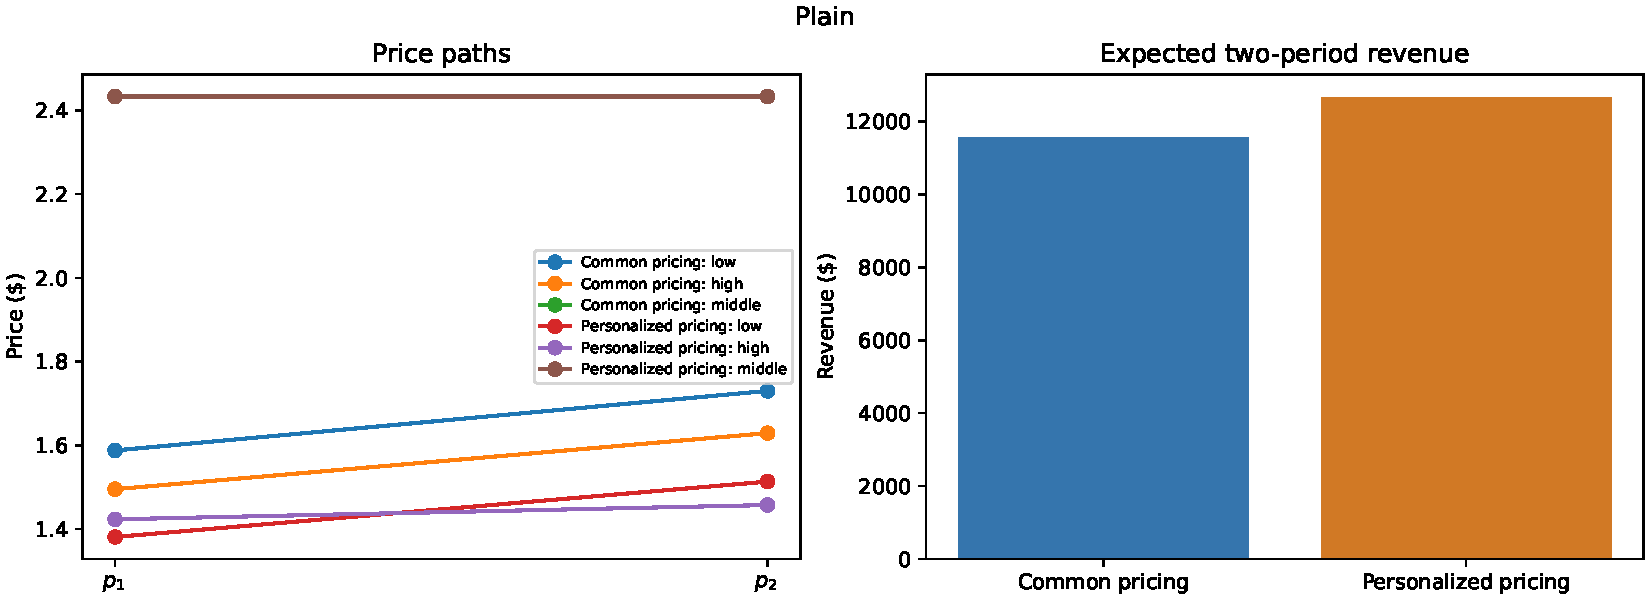
\includegraphics[width=\textwidth]{assets/pricing/plain/household_coupon_results.pdf}
\end{frame}


% Original numbered slide 38
\gdef\shortbuttons{\hyperlink{short-42}{\beamergotobutton{Back to Plain: Price Paths}}}
\begin{frame}[label=short-38,noframenumbering]{Berry: Optimal Offers by Consumer Type}
  \centering
  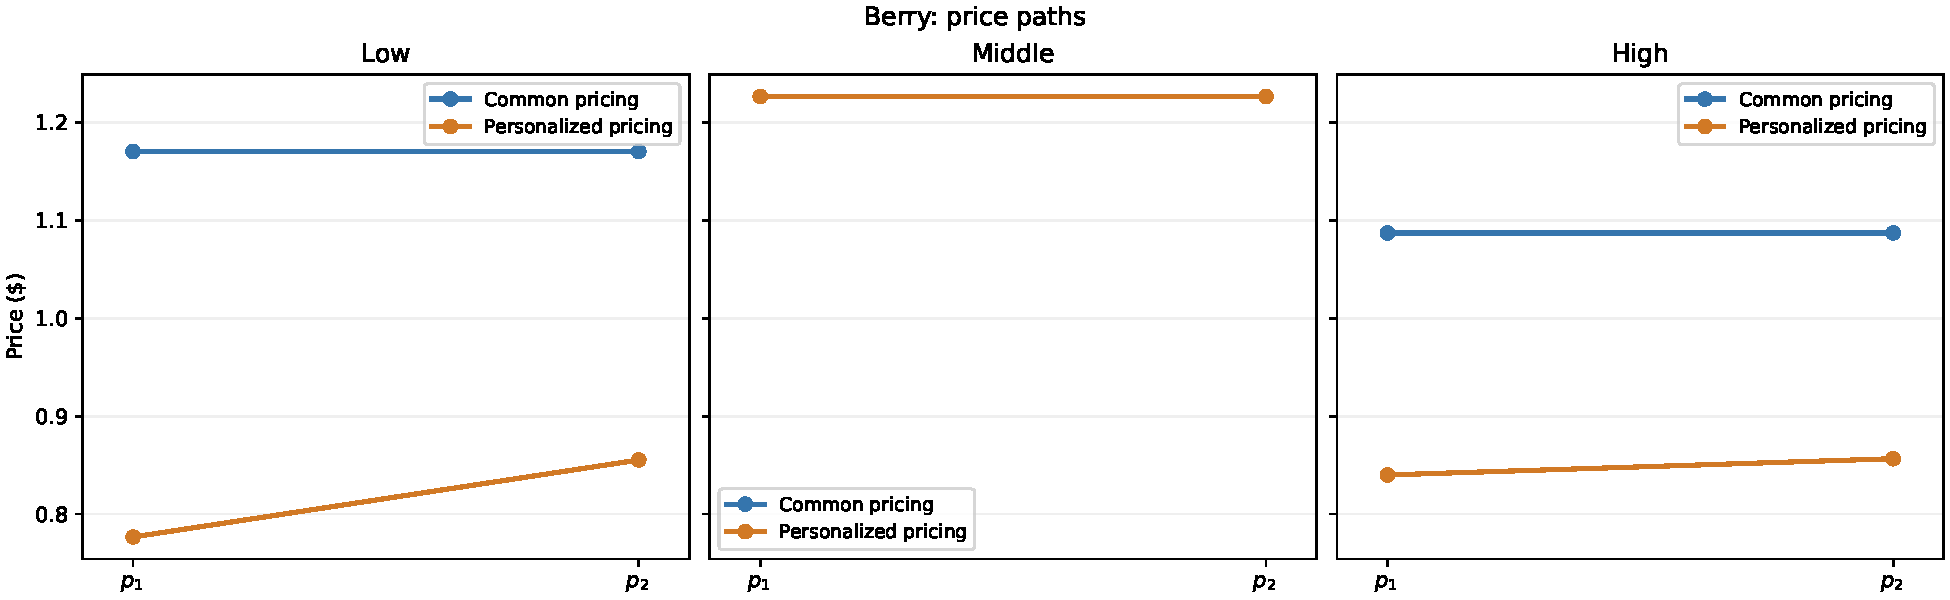
\includegraphics[width=0.85\textwidth]{assets/pricing/berry/discounts_by_consumer_type.pdf}
\end{frame}


% Original numbered slide 39
\gdef\shortbuttons{\hyperlink{short-42}{\beamergotobutton{Back to Plain: Price Paths}}}
\begin{frame}[label=short-39,noframenumbering]{Plain: Optimal Offers by Consumer Type}
  \centering
  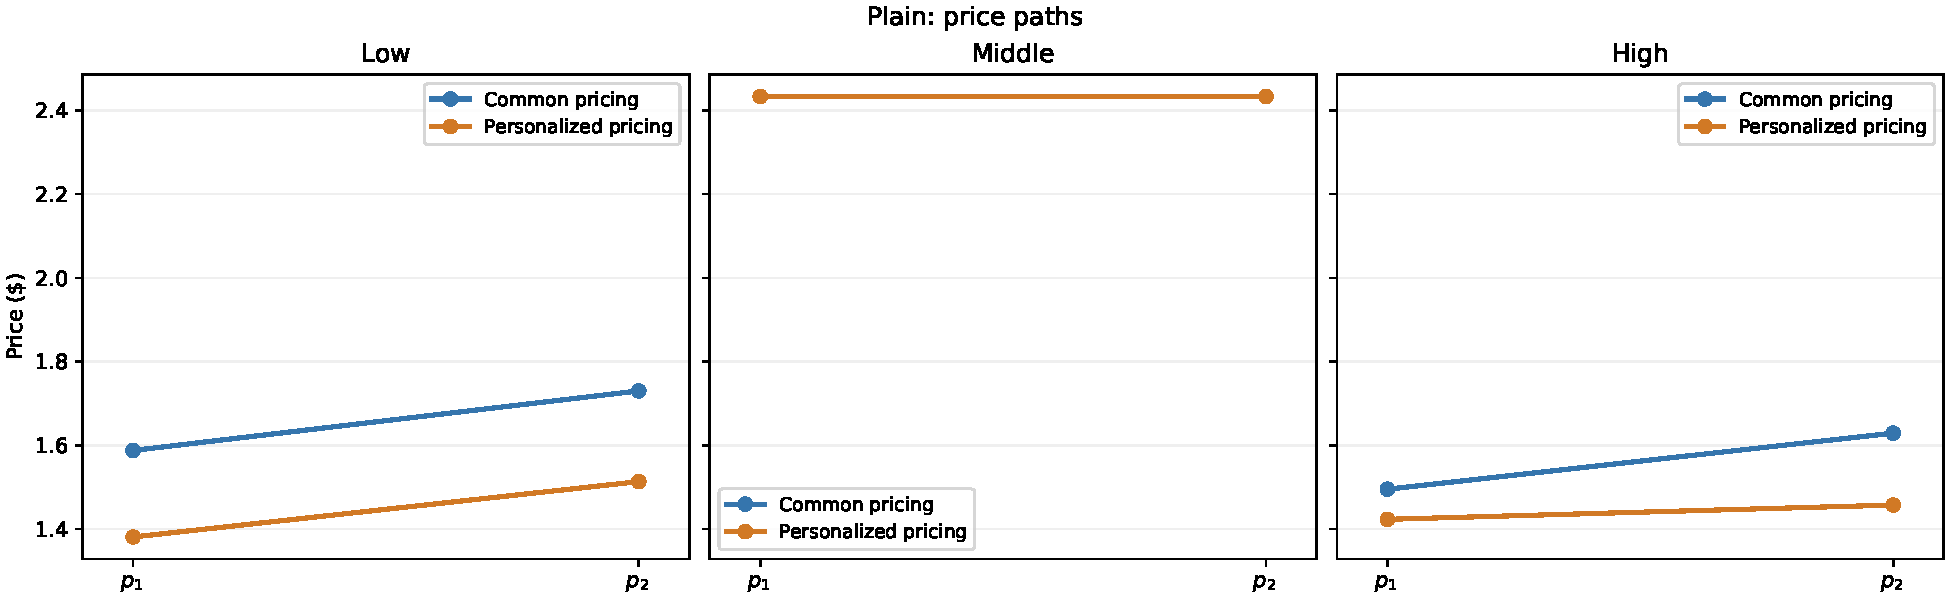
\includegraphics[width=0.85\textwidth]{assets/pricing/plain/discounts_by_consumer_type.pdf}
\end{frame}


\end{document}
